%\begin{center}
%\includegraphics[scale=0.05, angle=-90]{figboga/remark.JPG}
%\end{center}
\documentclass{article}
\usepackage[utf8]{inputenc}
\usepackage{amsmath}
\usepackage{xcolor}
\newcommand{\red}[1]{\textcolor{red}{#1}}
\usepackage{hyperref}
\usepackage{amsfonts}
\usepackage{listings}
\usepackage{color}
\definecolor{dkgreen}{rgb}{0,0.6,0}
\definecolor{gray}{rgb}{0.5,0.5,0.5}
\definecolor{mauve}{rgb}{0.58,0,0.82}
\lstset{frame=tb,
  language=Python,
  aboveskip=3mm,
  escapechar=\%,
  belowskip=3mm,
  showstringspaces=false,
  columns=flexible,
  basicstyle={\small\ttfamily},
  numbers=none,
  numberstyle=\tiny\color{black},
  keywordstyle=\color{black},
  commentstyle=\color{dkgreen},
  stringstyle=\color{black},
  breaklines=true,
  breakatwhitespace=true,
  tabsize=3
}
\usepackage{ mathrsfs }
\usepackage{amsthm}
\usepackage{amssymb}
\usepackage{graphics}
\usepackage{graphicx}
\usepackage{tikz-cd}
\usepackage{mathtools}
\usepackage{booktabs}
\DeclareMathOperator\dom{dom}
\DeclareMathOperator\vphi{\varphi}
\DeclareMathOperator\eps{\epsilon}
\DeclareMathOperator\del{\delta}
\DeclareMathOperator\Del{\Delta}
\DeclareMathOperator\lm{\lambda}
\DeclareMathOperator\deq{\vcentcolon=}
\DeclareMathOperator\R{\mathbb{R}}
\DeclareMathOperator\pr{\mathbb{P}}
\DeclareMathOperator\Z{\mathbb{Z}}
\DeclareMathOperator\N{\mathbb{N}}
\DeclareMathOperator\F{\mathbb{F}}
\DeclareMathOperator\A{\mathbb{A}}
\DeclareMathOperator\HH{\mathbb{H}}
\DeclareMathOperator\minn{\text{Minimise} \quad }
\DeclareMathOperator\maxx{\text{Maximise} \quad }
\DeclareMathOperator\st{\text{Subject to} \quad }
\DeclareMathOperator\nc{\text{no constraints}}
\DeclarePairedDelimiter\ceil{\lceil}{\rceil}
\DeclarePairedDelimiter\floor{\lfloor}{\rfloor}
\DeclareMathOperator\bx{\bold{x}}
\DeclareMathOperator\bs{\bold{s}}
\DeclareMathOperator\id{\text{Id}}
\DeclareMathOperator\bb{\bold{b}}
\DeclareMathOperator\bA{\bold{A}}
\DeclareMathOperator\bp{\bold{p}}
\DeclareMathOperator\bc{\bold{c}}
\DeclareMathOperator\C{\mathbb{C}}
\DeclareMathOperator\ran{ran}
\DeclareMathOperator\img{Im}
\DeclareMathOperator\op{\oplus}
\DeclareMathOperator\ot{\otimes}
\DeclareMathOperator\diam{diam}
\DeclareMathOperator\ite{int}
\DeclareMathOperator*{\argmax}{arg\,max}
\DeclareMathOperator*{\argmin}{arg\,min}
\DeclareMathOperator\cd{card}
\DeclareMathOperator\la{\langle}
\DeclareMathOperator\ra{\rangle}
\DeclareMathOperator\erf{erf}
\DeclareMathOperator\erfc{erfc}
\DeclareMathOperator\iso{\,\simeq\,}
\DeclareMathOperator{\sgn}{sgn}
\DeclareMathOperator{\lcm}{lcm}

\newtheorem{lemma}{Lemma}
\newtheorem{theorem}{Theorem}
\newtheorem{cor}{Corollary}
\newcommand{\an}[1]{\langle \, #1 \, \rangle}
\newcommand{\GL}{\text{GL}(\mathbb{R}^n)}
\newcommand{\GLM}{\text{GL}(n,\mathbb{R})}
\newcommand{\quo}{/ _\sim}
\newcommand{\phii}{\phi^{-1}}
\newcommand{\pa}{\partial}
\newcommand{\lb}{\left}
\newcommand{\rb}{\right}
\newcommand{\aps}{\alpha_S}
\newcommand{\apl}{\alpha_L}
\newcommand{\tdd}{\frac{d^2T}{dx^2}}
\newcommand{\dx}{\frac{d}{dx}}
\newcommand{\seq}{(x_n)_{n \geq 1}}
\newcommand{\sseq}{(x_{n_k})_{k \geq 1}}
\newcommand{\fseq}{(f_n)_{n \geq 1}}
\newcommand{\elll}{\ell^{\infty}(\N)}
\newcommand{\norm}{{\|.\|}}
\newcommand{\inner}{\langle .,. \rangle}
\newcommand*\dd{\, \mathop{}\!\mathrm{d}}
\newcommand*\DD[1]{\, \mathop{}\!\mathrm{d^#1}}
\newcommand{\Ga}[1]{\frac{1}{\sqrt{2\pi\sigma^2}} e^{-\frac{\left(#1\right)^2}{2\sigma^2}}}
\usepackage{color}
%\title{}
\newcommand*\autoop{\left(}
\newcommand*\autocp{\right)}
\newcommand*\autoob{\left[}
\newcommand*\autocb{\right]}
\DeclareRobustCommand*\{{\ifmmode \left\lbrace \else \textbraceleft \fi }
\DeclareRobustCommand*\}{\ifmmode \right\rbrace \else \textbraceright \fi }
\AtBeginDocument {%
   \mathcode`( 32768
   \mathcode`) 32768
   \mathcode`[ 32768
   \mathcode`] 32768
   \begingroup
       \lccode`\~`(
       \lowercase{%
   \endgroup
       \let~\autoop
   }\begingroup
       \lccode`\~`)
       \lowercase{%
   \endgroup
       \let~\autocp
   }\begingroup
       \lccode`\~`[
       \lowercase{%
   \endgroup
       \let~\autoob
   }\begingroup
       \lccode`\~`]
       \lowercase{%
   \endgroup
       \let~\autocb
   }}

\delimiterfactor 1001

\makeatletter
% for amsmath "compatibility" (not sophisticated)
% \usepackage{amsmath}
\AtBeginDocument {%
          \def\resetMathstrut@{%
           \setbox\z@\hbox{\the\textfont\symoperators\char40}%
           \ht\Mathstrutbox@\ht\z@ \dp\Mathstrutbox@\dp\z@}%
}%
\makeatother
\author{Brendan Matthews}
\title{A First Course in Abstract Algebra}
\begin{document}
\maketitle{}
\newpage{}
\section*{Chapter -2: What is this stuff used for}
\begin{tabular}{cccc}
\hline
\textbf{Topic} & \textbf{It is used} & \textbf{What Part} & \textbf{Is it Physics} \\
\hline
Combinatorics & yes & Group Actions: Burnside & no\\
Statistics & sparsely & Renormalisation group, Haar Measure & yes, dunno  \\
Statistics &sparsely & Galois Fields: Fractional factorial design & no \\
Math &&& \\
Math &&& \\
Math &&& \\
Math &&& \\
\hline
\end{tabular}
\section*{Chapter -1}
Group tables are dumb and playing sudoku doesn't guarantee associativity.
\begin{center}
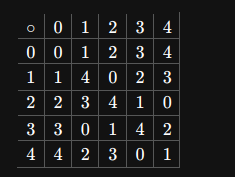
\includegraphics[scale=0.6, angle=-0]{fig/countergroup.png}
\end{center}
$D_3 = S_3$ but $D_n \neq S_n, \quad n \geq 4$.
\begin{center}
\includegraphics[scale=0.6, angle=-90]{fig/IMG_7240.jpeg}
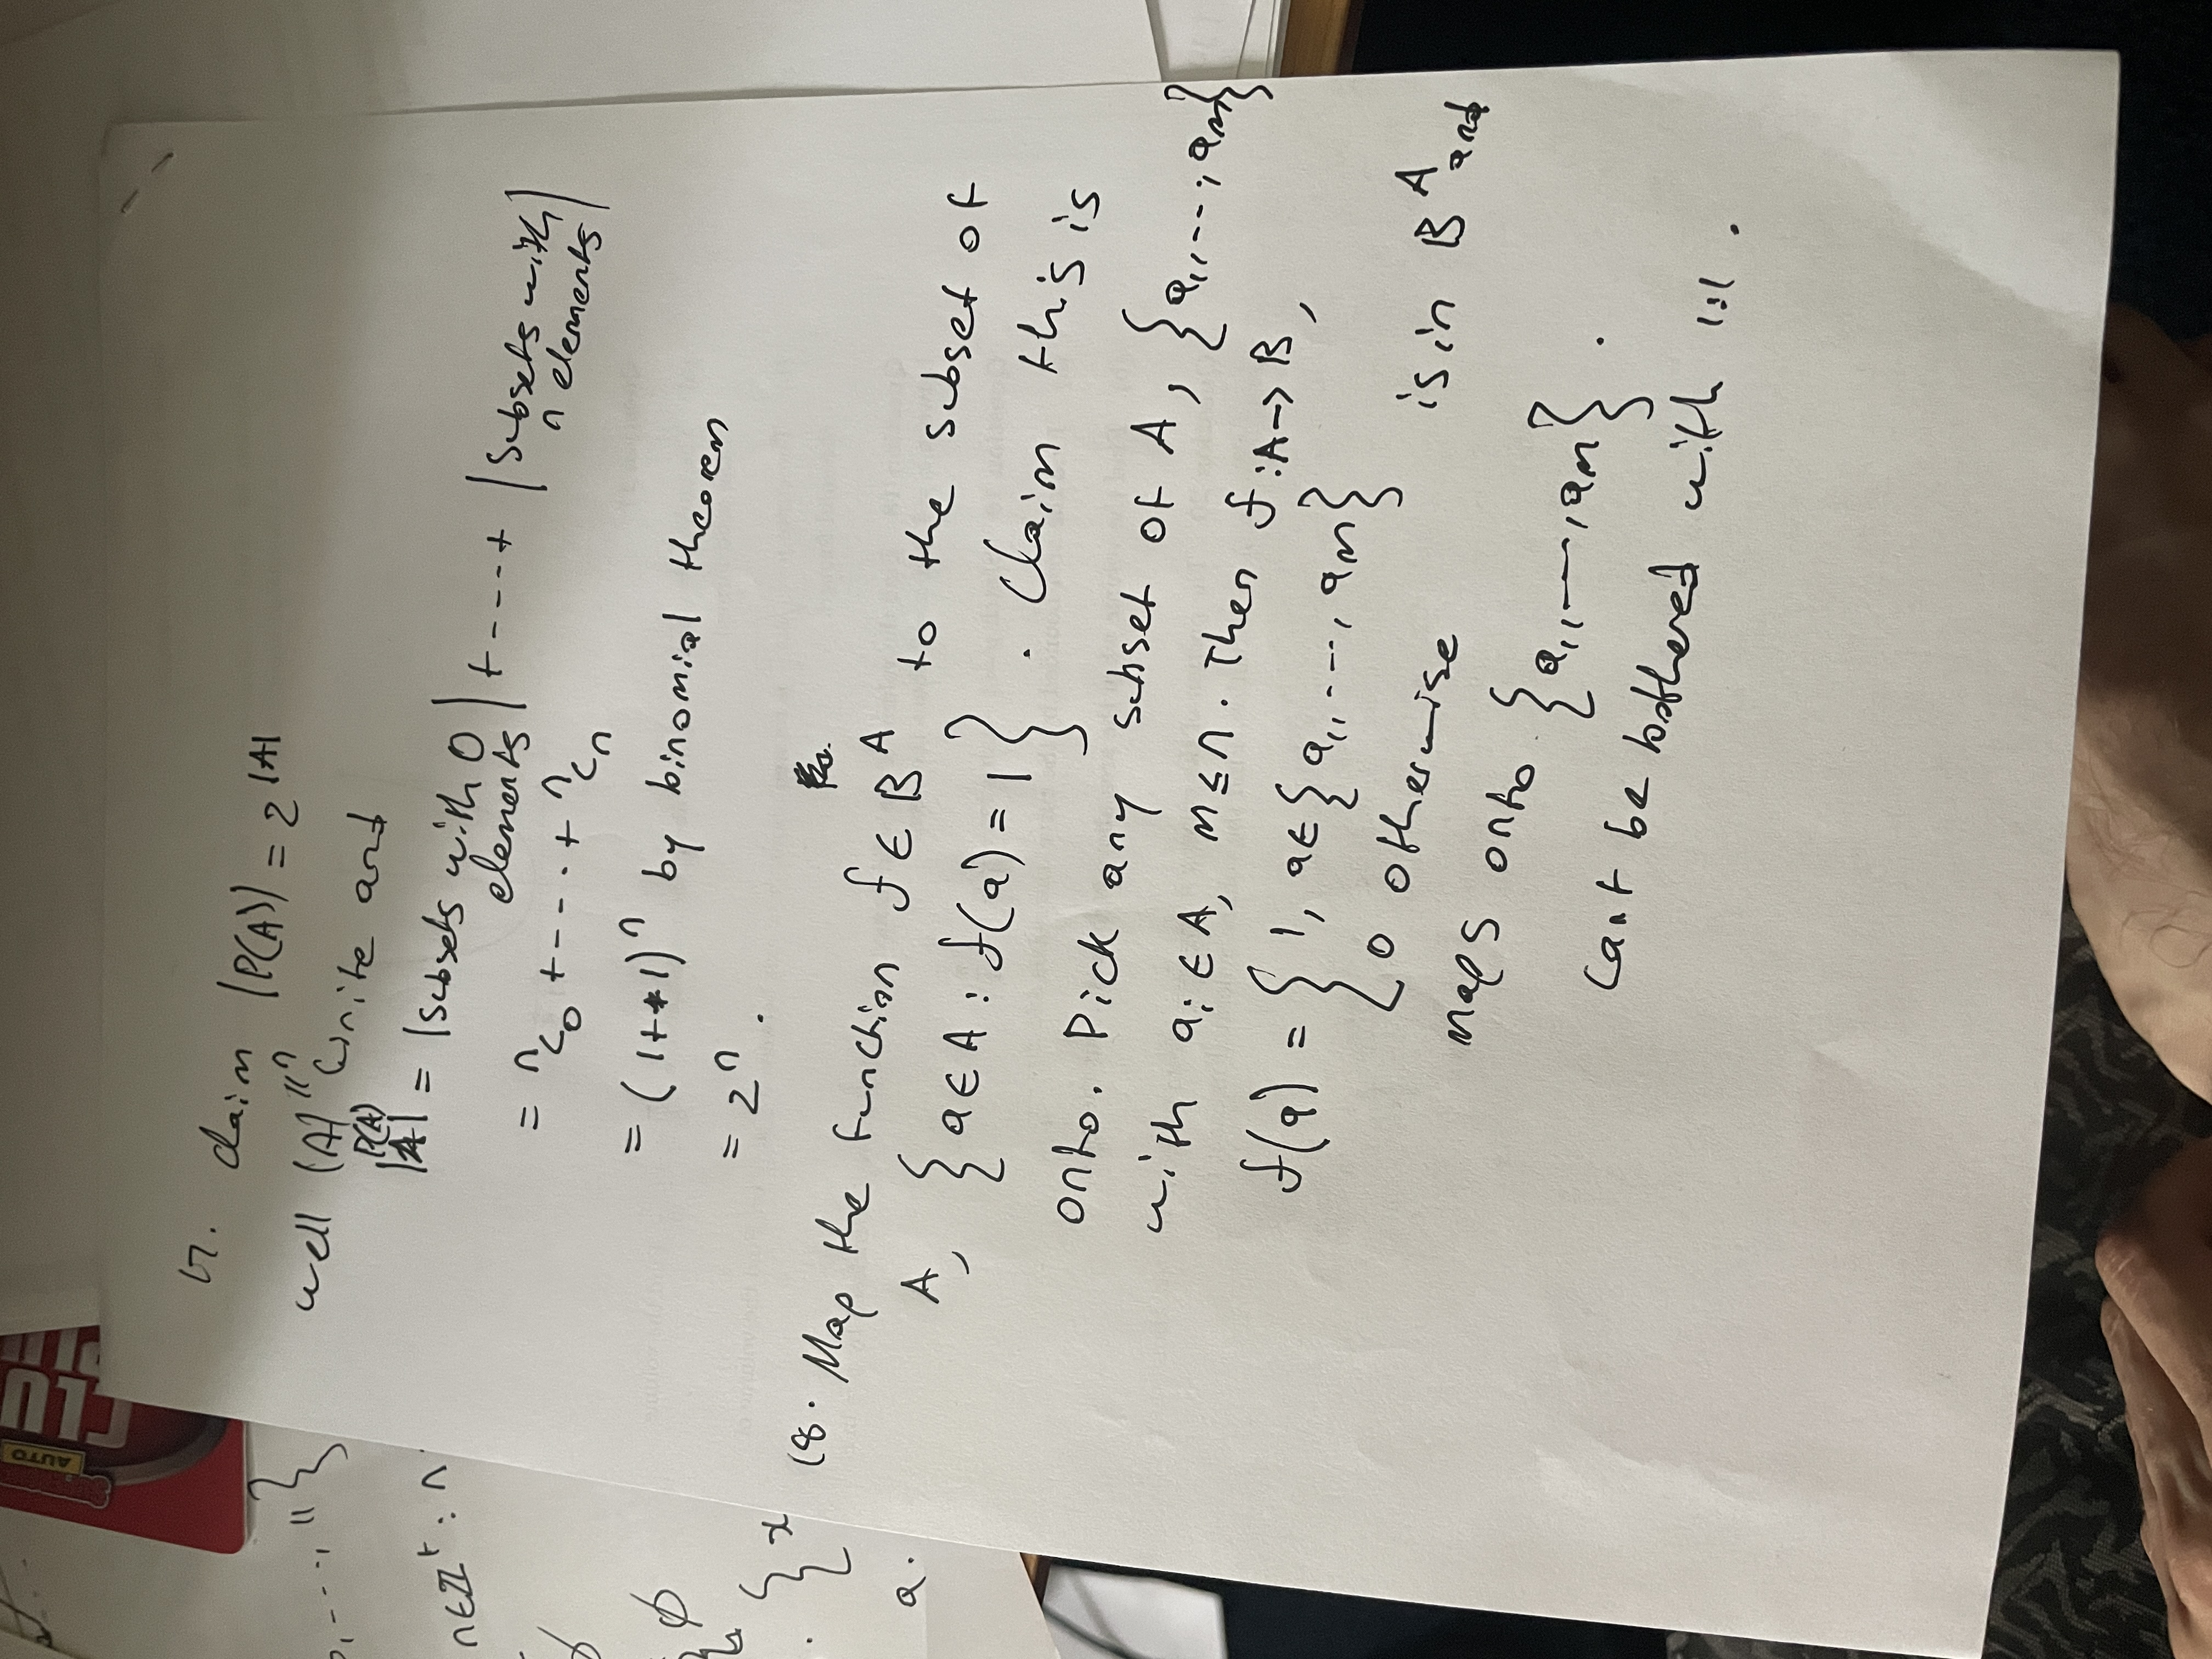
\includegraphics[scale=0.6, angle=-90]{fig/IMG_7241.jpeg}
\end{center}
\section{}
A binary operation is a map $*:S \times S \to S$ and a subset $H$ of $S$ is closed under $*$ if the obvious thing happens.
We say that $*$ is induced on $H$. There are $n^{n^2}$ binary ops on a set of size $n$ and $n^{\sum_n i} = n^{\frac{n(n+1)}{2}}$ commutative ones.
The latter is because the number of elements of $S \times S$ that aren't predetermined by the condition is $n+(n-1)+\hdots+1$ and schoolboy Gauss does the rest.
Note that for finite $A,B$, number of maps from $A$ to $B$ is $|B|^{|A|}$.
\begin{center}
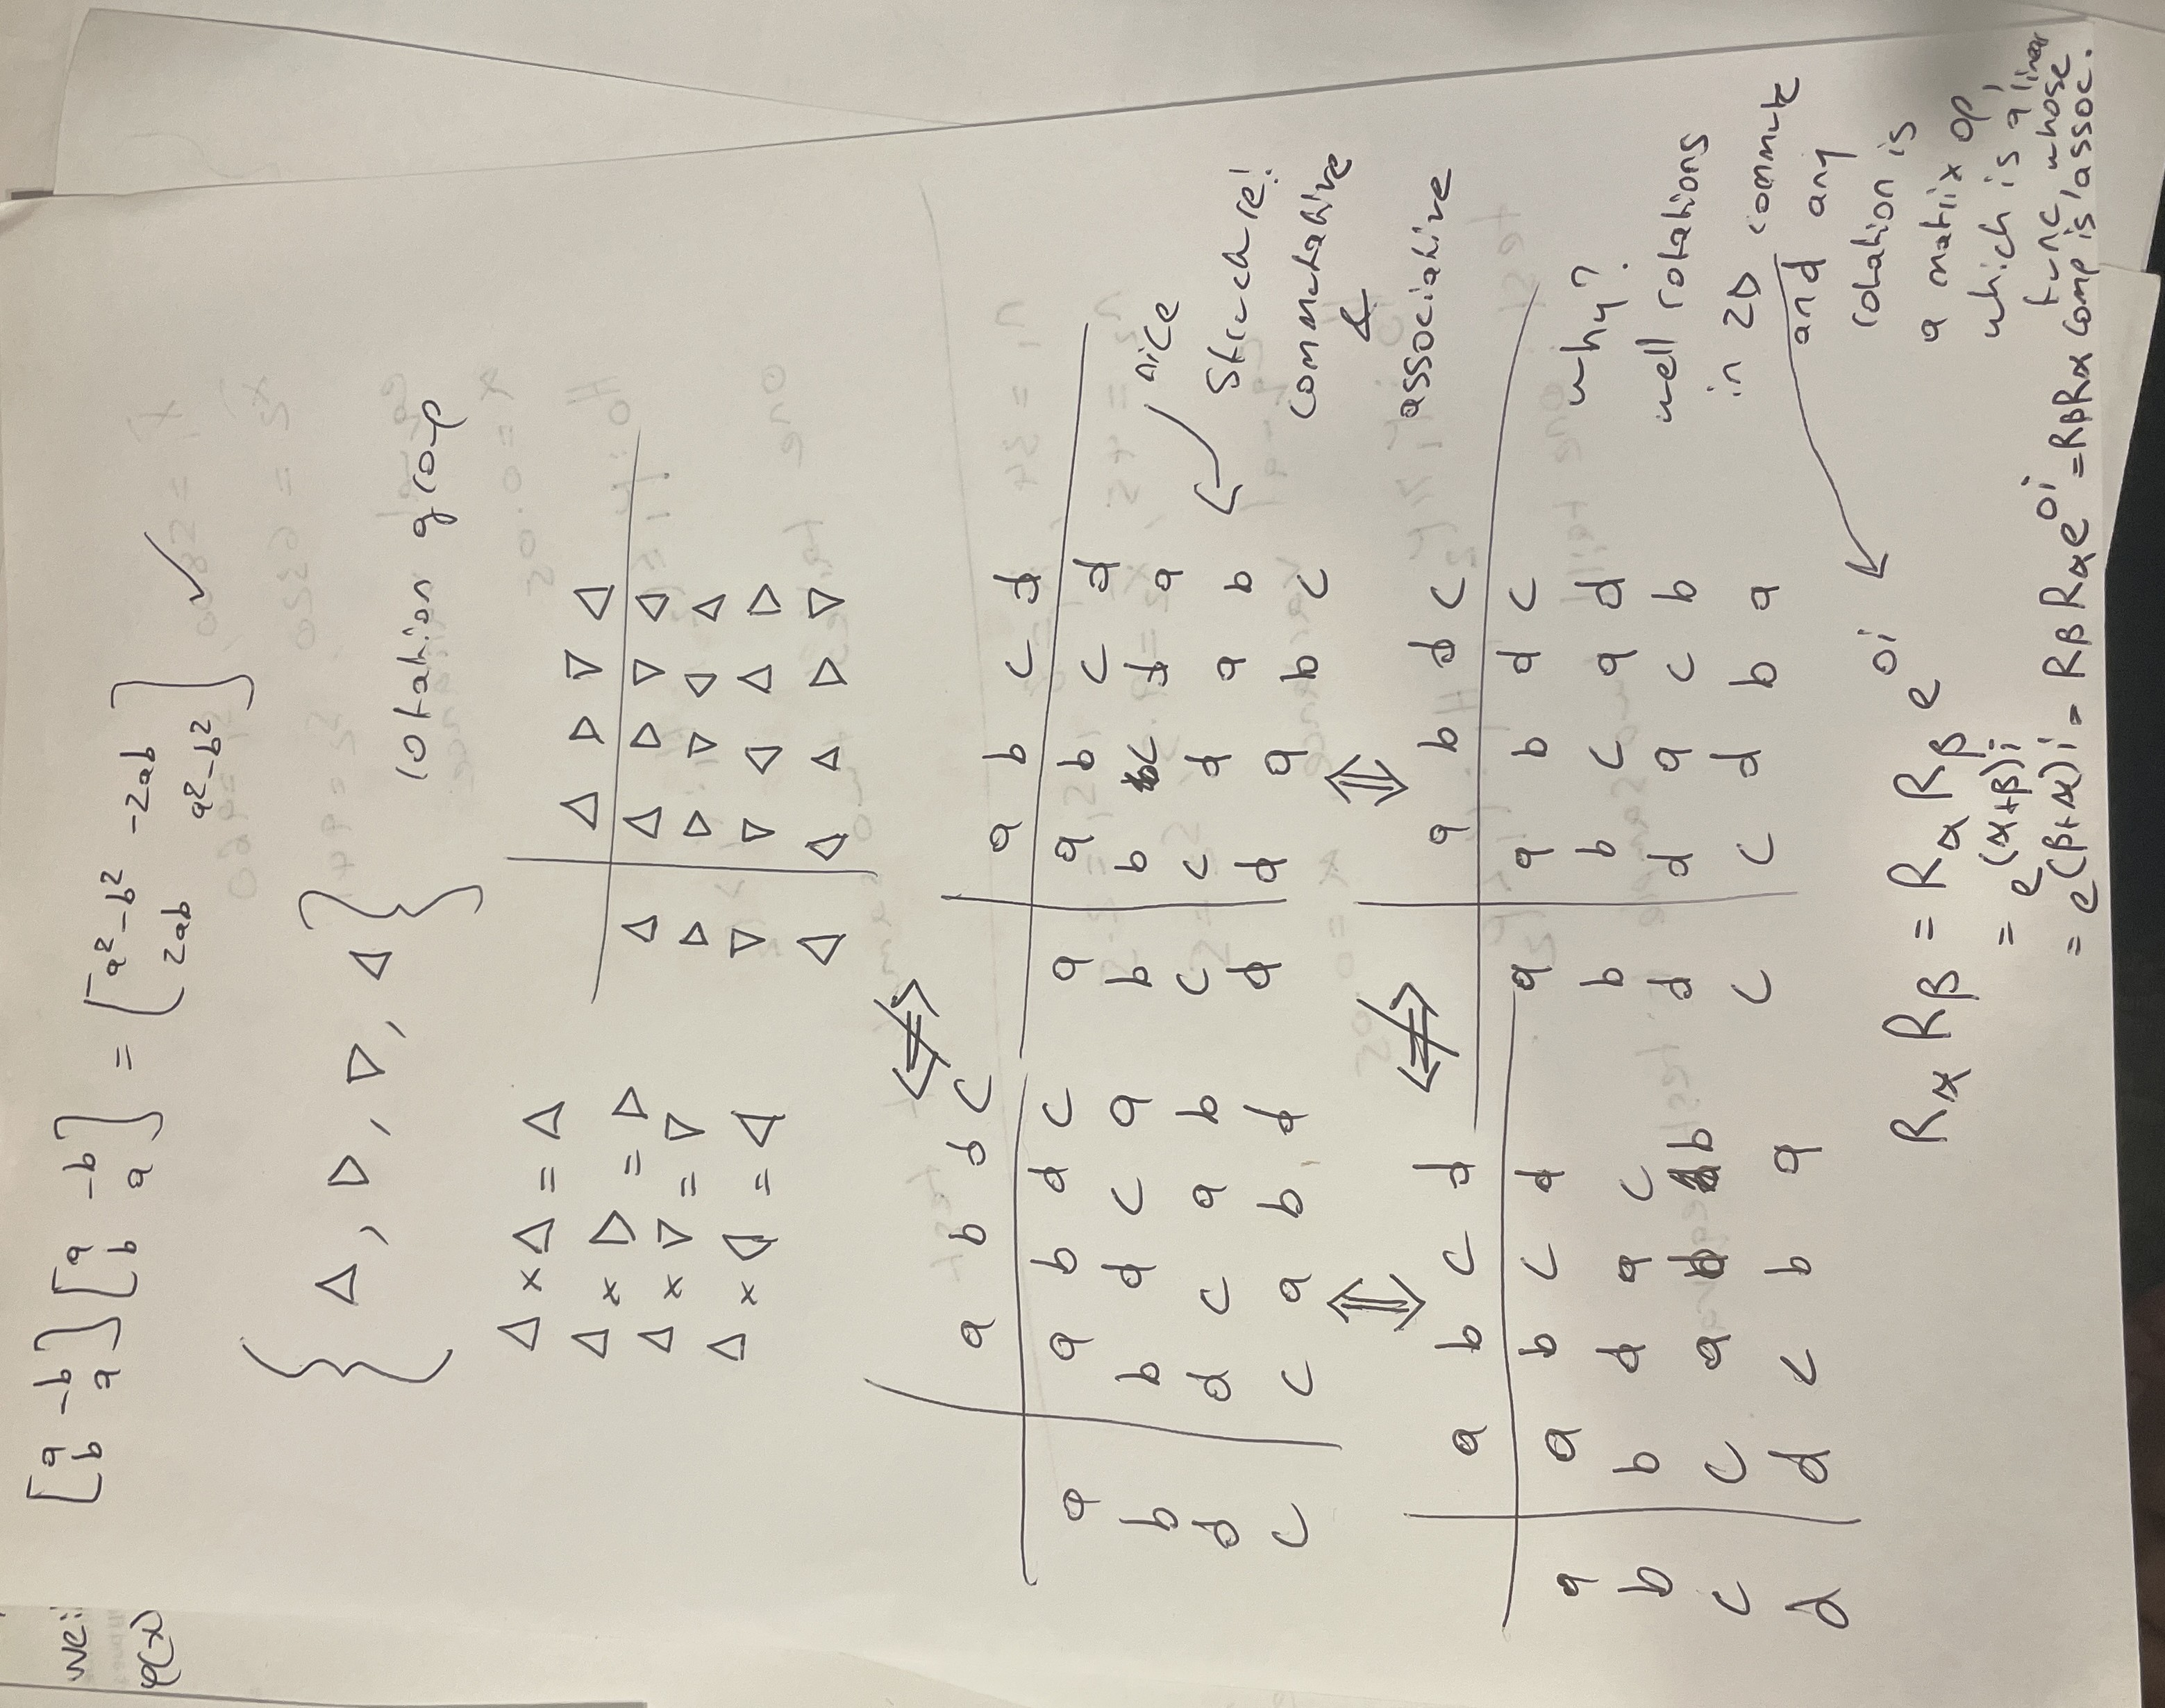
\includegraphics[scale=0.1, angle=-90]{fig/IMG_7243.jpeg}
\end{center}
Not every 2 element commuter is associative. Consider $aa = b, \,\, ab=b,\,\,ba=b,\,\,bb=a$ and $a(ab) = ab=b,\,\,(aa)b=bb=a$. 35 is rubbish.
\begin{center}
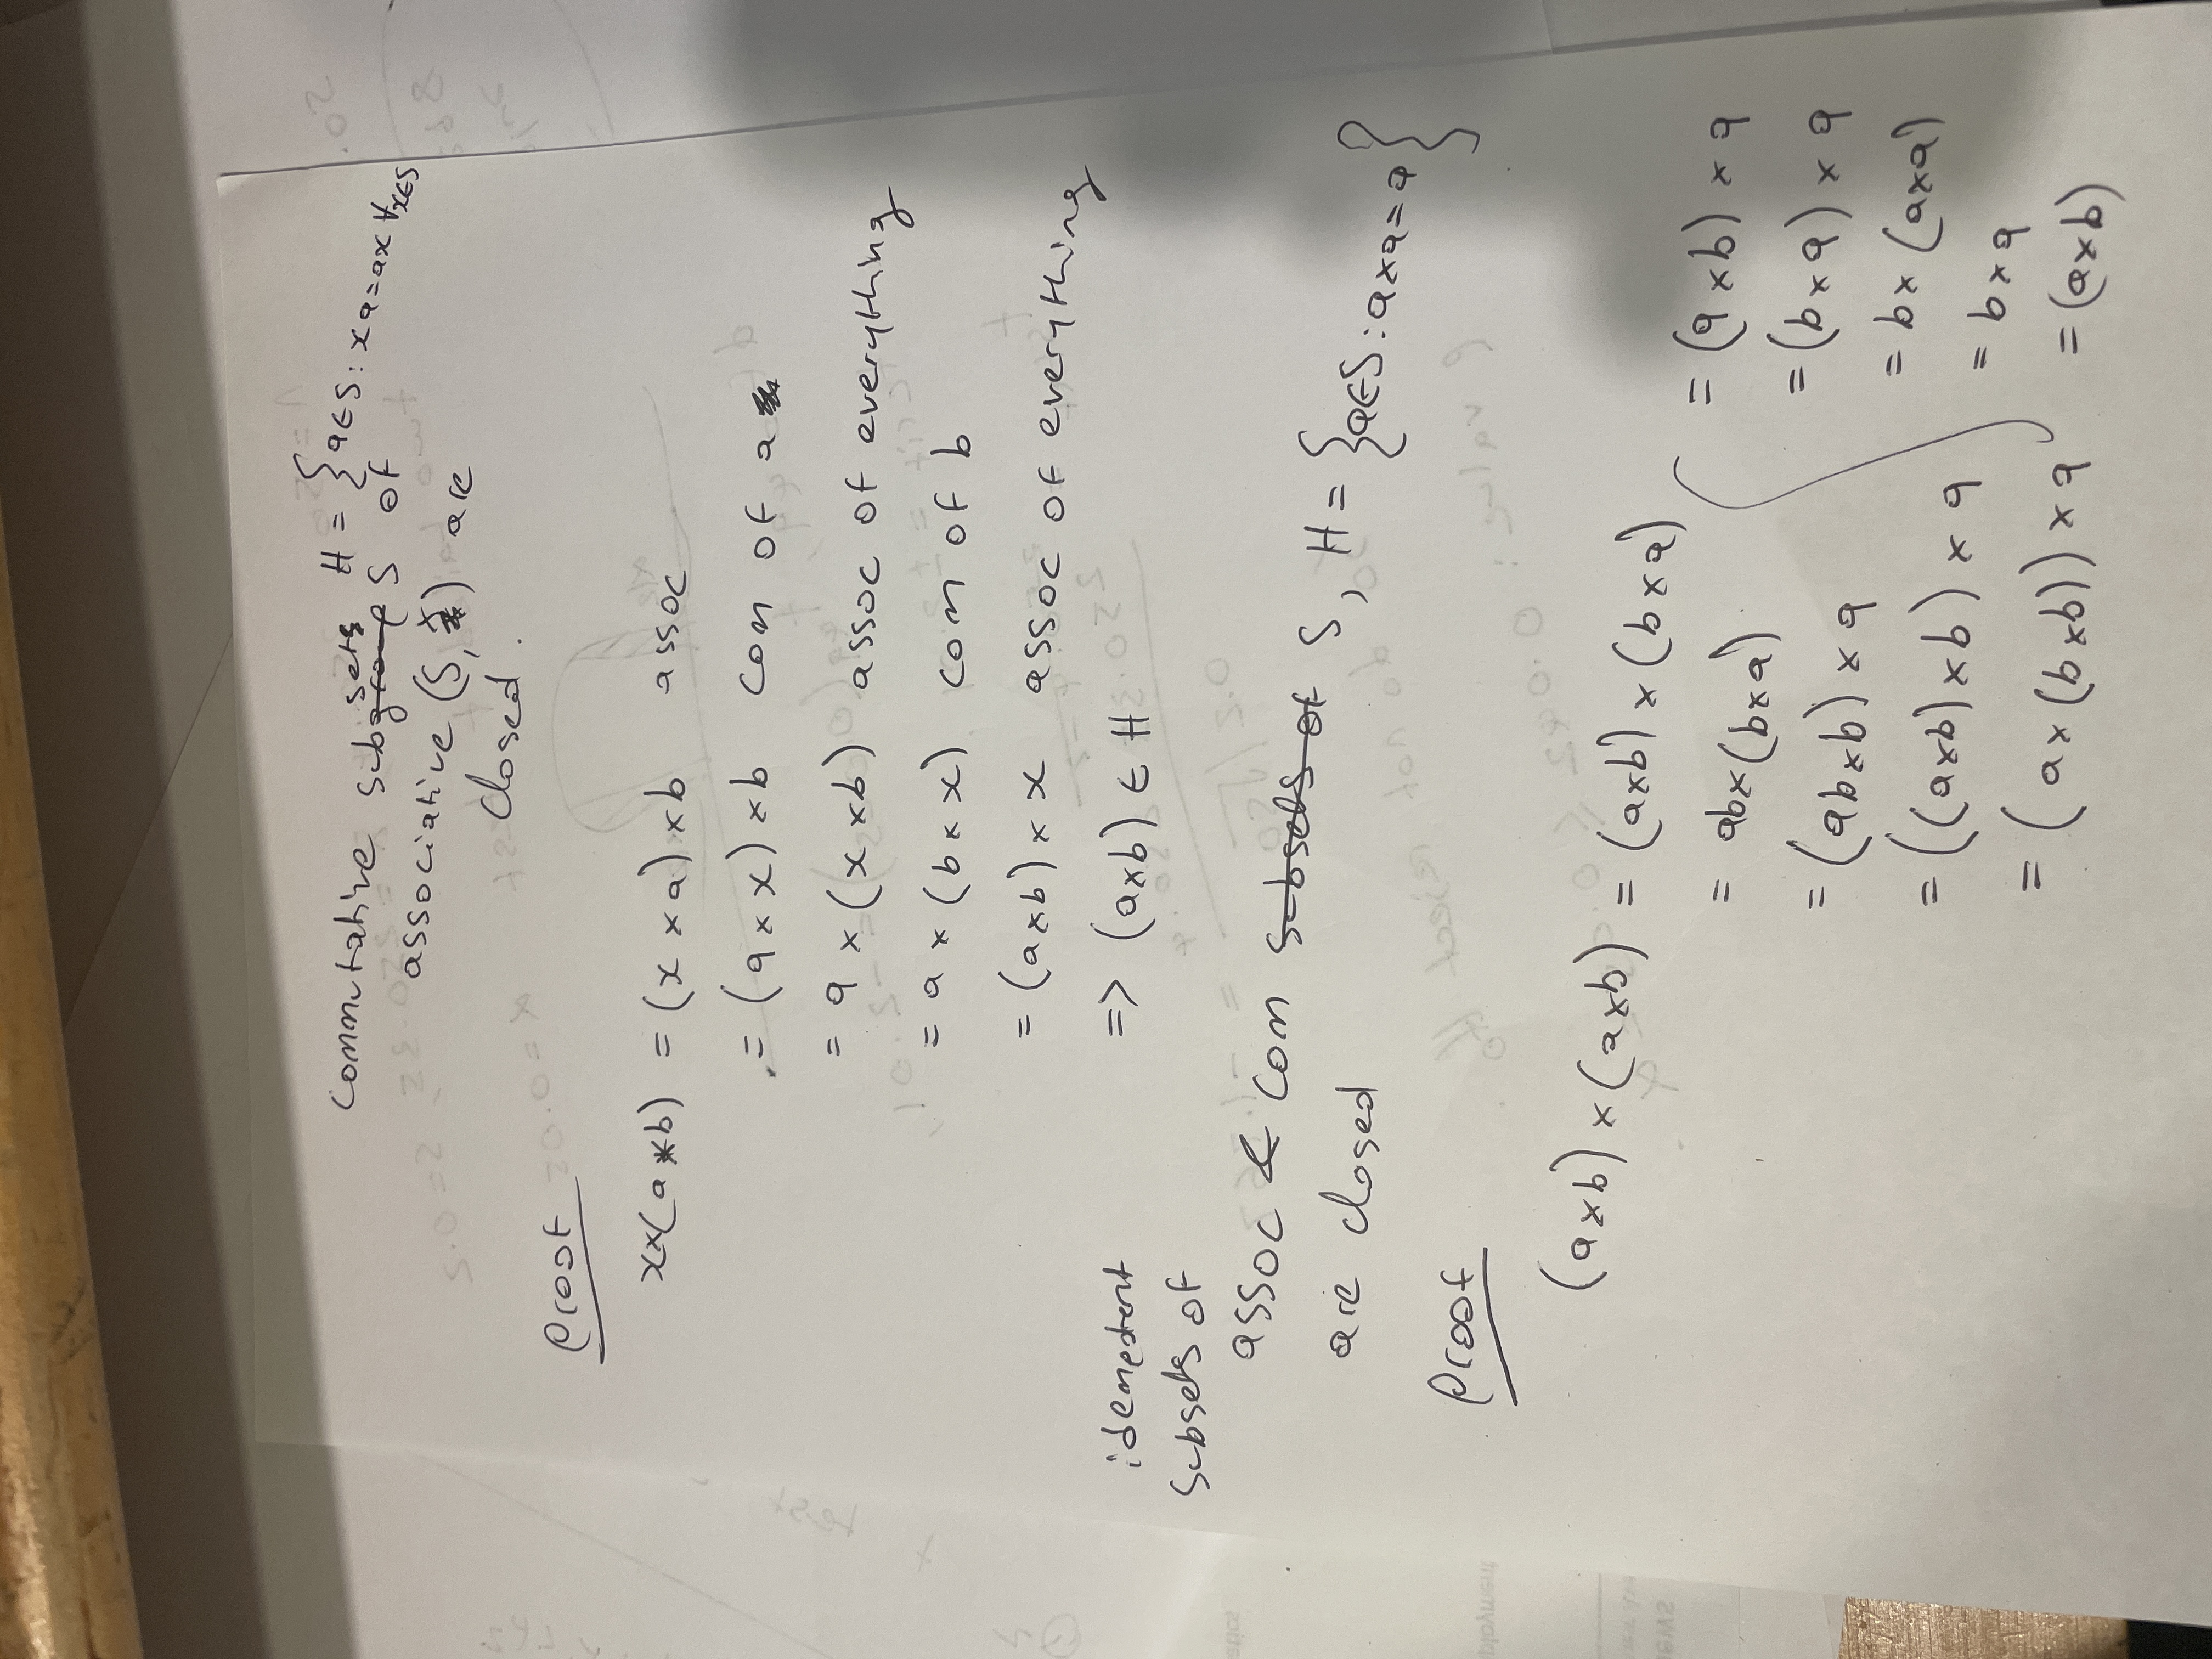
\includegraphics[scale=0.4, angle=-90]{fig/IMG_7244.jpeg}
\end{center}
\section*{}
Two binary algebraic structures $(R,*),(S,+)$ are isomorphic, $R \iso S$, if for each $x,y \in R$ with $x*y = z$,
we have corresponding $x',y',z' \in S$ so that $x' + y' = z'$. That is,
there exists a bijection $\phi:R \to S$ such that for all $x,y \in R$ with $x*y=z$,
\[
\phi(x*y) = \phi(x)+\phi(y) = x'+y' = z' = \phi(z).
\]
Each point in $S$ is mapped to by exactly one point in $R$. Isomorphism is an equivalence relation.
\begin{proof}
$S \iso S$ by identity map. If $R \iso S$, then there exists $\phi:R \to S$, bijective and a homomorphism. So the inverse exists.
The inverse is a homomorphism by injectivity of $\phi$: $$
\phi(\phii(s_1)*\phii(s_2)) \underset{\text{H prop of $\phi$}}{=} \phi(\phii(s_1))+\phi(\phii(s_2)) = s_1 + s_2 = \phi(\phii(s_1+s_2)).
$$
Transitivity is easy just compose the isos.
\end{proof}
\subsection*{Theorem}
Suppose there is an onto homomorphism $\phi:(R,+) \to (S,*)$ and an identity $e \in R$. Then $\phi(e) \in S$ is an identity.
\begin{proof}
Easy.
\end{proof}
Note that while the identity is always unique in $S$, we require that $\phi$ be an isomorphism for the preimage of the identity to be uniquely the identity of $R$.
\subsection*{Theorem}
Suppose $S$ is a \textbf{group} and $R,S$ have identities $e_R,e_S$. If there is a homomorphism $\phi:(R,+) \to (S,*)$, then $\phi(e_R) = e_S$.
\begin{proof}
$$
\phi(e_R) = \phi(e_R+e_R) = \phi(e_R) * \phi(e_R)
$$
Apply inverse of $\phi(e_R)$.
\end{proof}
\subsection*{Non Isomorphism Example}
The function $\phi: (M_2(\R),\times) \to (\R,\times), \quad \phi(A) = \det(A)$ is not an isomorphism (in fact, no such isomorphism exists).
\begin{proof}
It is a homomorphism, $\det(AB) = \det(A)\det(B)$. But it isn't injective because matrix multiplication isn't commutative.
Take $$A = \begin{bmatrix}
1 & 1 \\
0 & 1
\end{bmatrix},\quad B =
\begin{bmatrix}
1 & 0 \\
1 & 1
\end{bmatrix}
$$
then $$
AB = \begin{bmatrix}
2 & 1 \\
1 & 1
\end{bmatrix},\quad BA =
\begin{bmatrix}
1 & 1 \\
1 & 2
\end{bmatrix}
$$
so that $$
\phi(AB) = \phi(BA) = 1 \text{ but } AB \neq BA.
$$
\end{proof}
\noindent Another example that fails injectivity is the map under addition from functions with derivatives to their derivatives.
Being a binary operation (or even a function at all) can fail with integrals even if everything else works.
\subsection*{Disproof using stuff that's preserved under isomorphisms}
We know the identity is preserved. So $\phi(f)(x) = xf(x)$ is not an isomorphism across $F = \{f: \R \to \R| f \text{ is smooth}\}$ under multiplication, $\phi(\bf{1})(2) = 2 \neq 1$, so $\phi(\bf{1}) \neq \bf{1}$, where $\bf{1}: \R \to \R$ is given by $\bf{1}$$ (x) = 1$.
\begin{center}
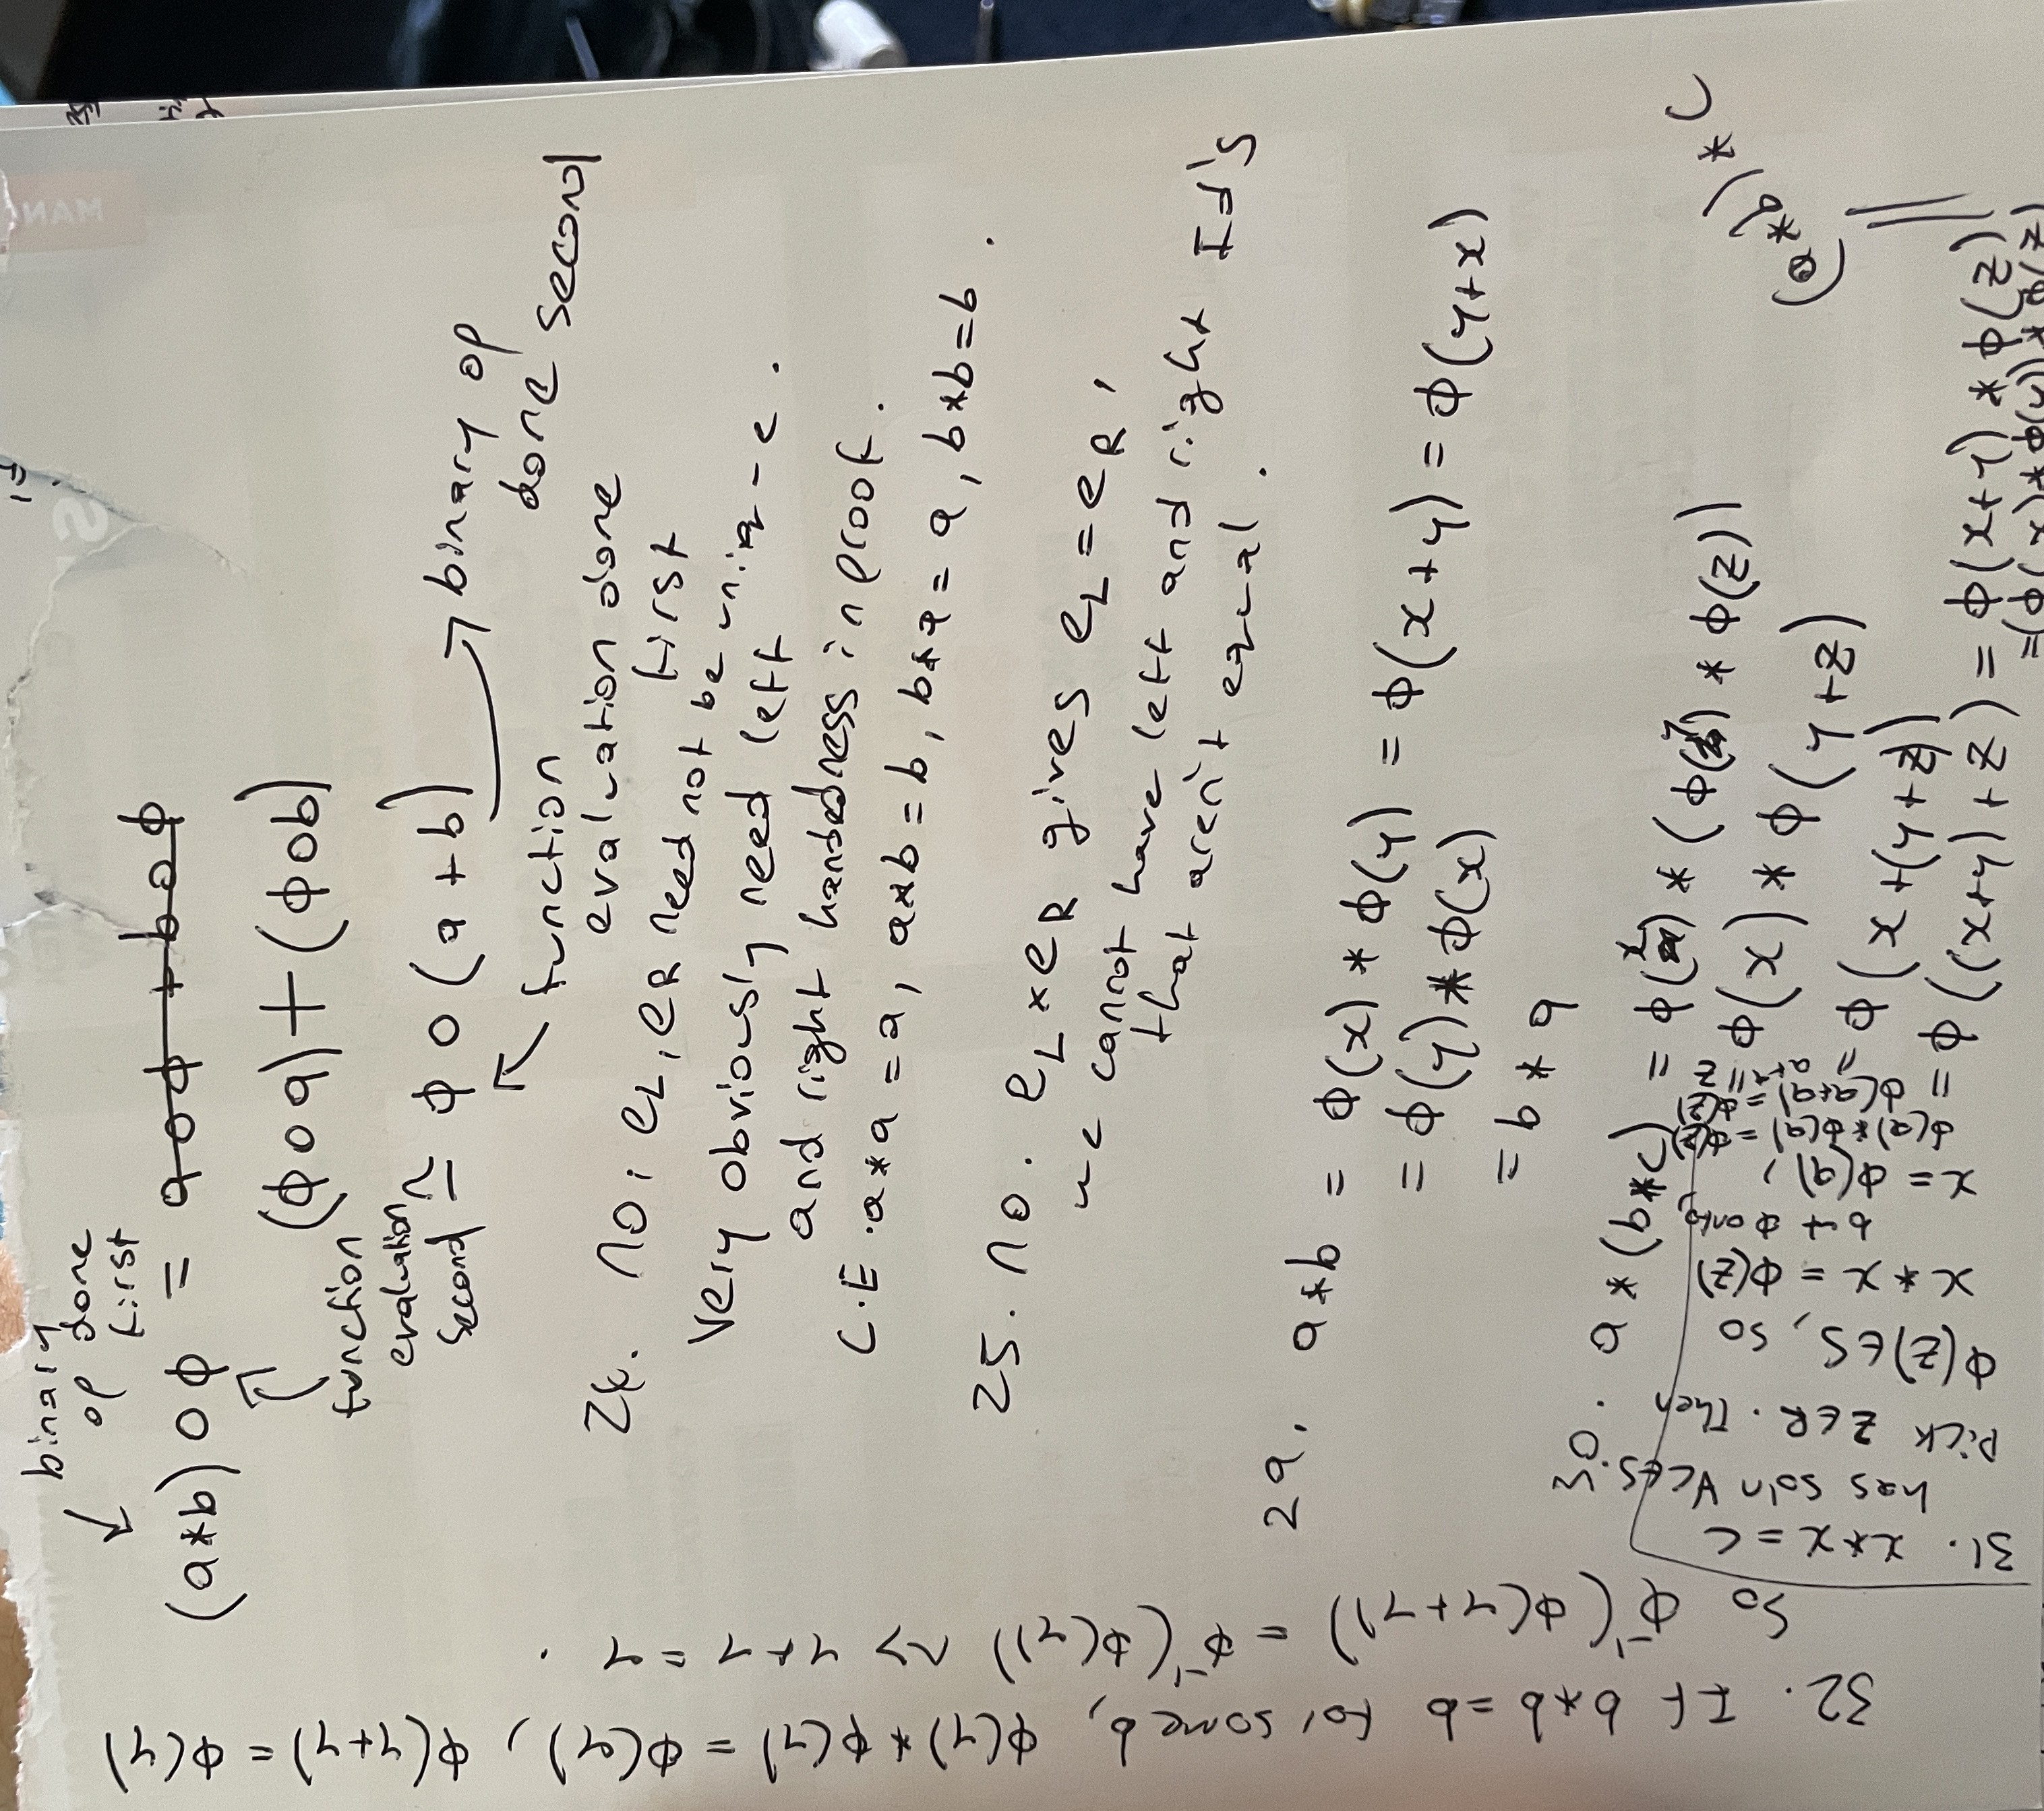
\includegraphics[scale=0.1, angle=-90]{fig/IMG_7271.jpeg}
\end{center}
\begin{center}
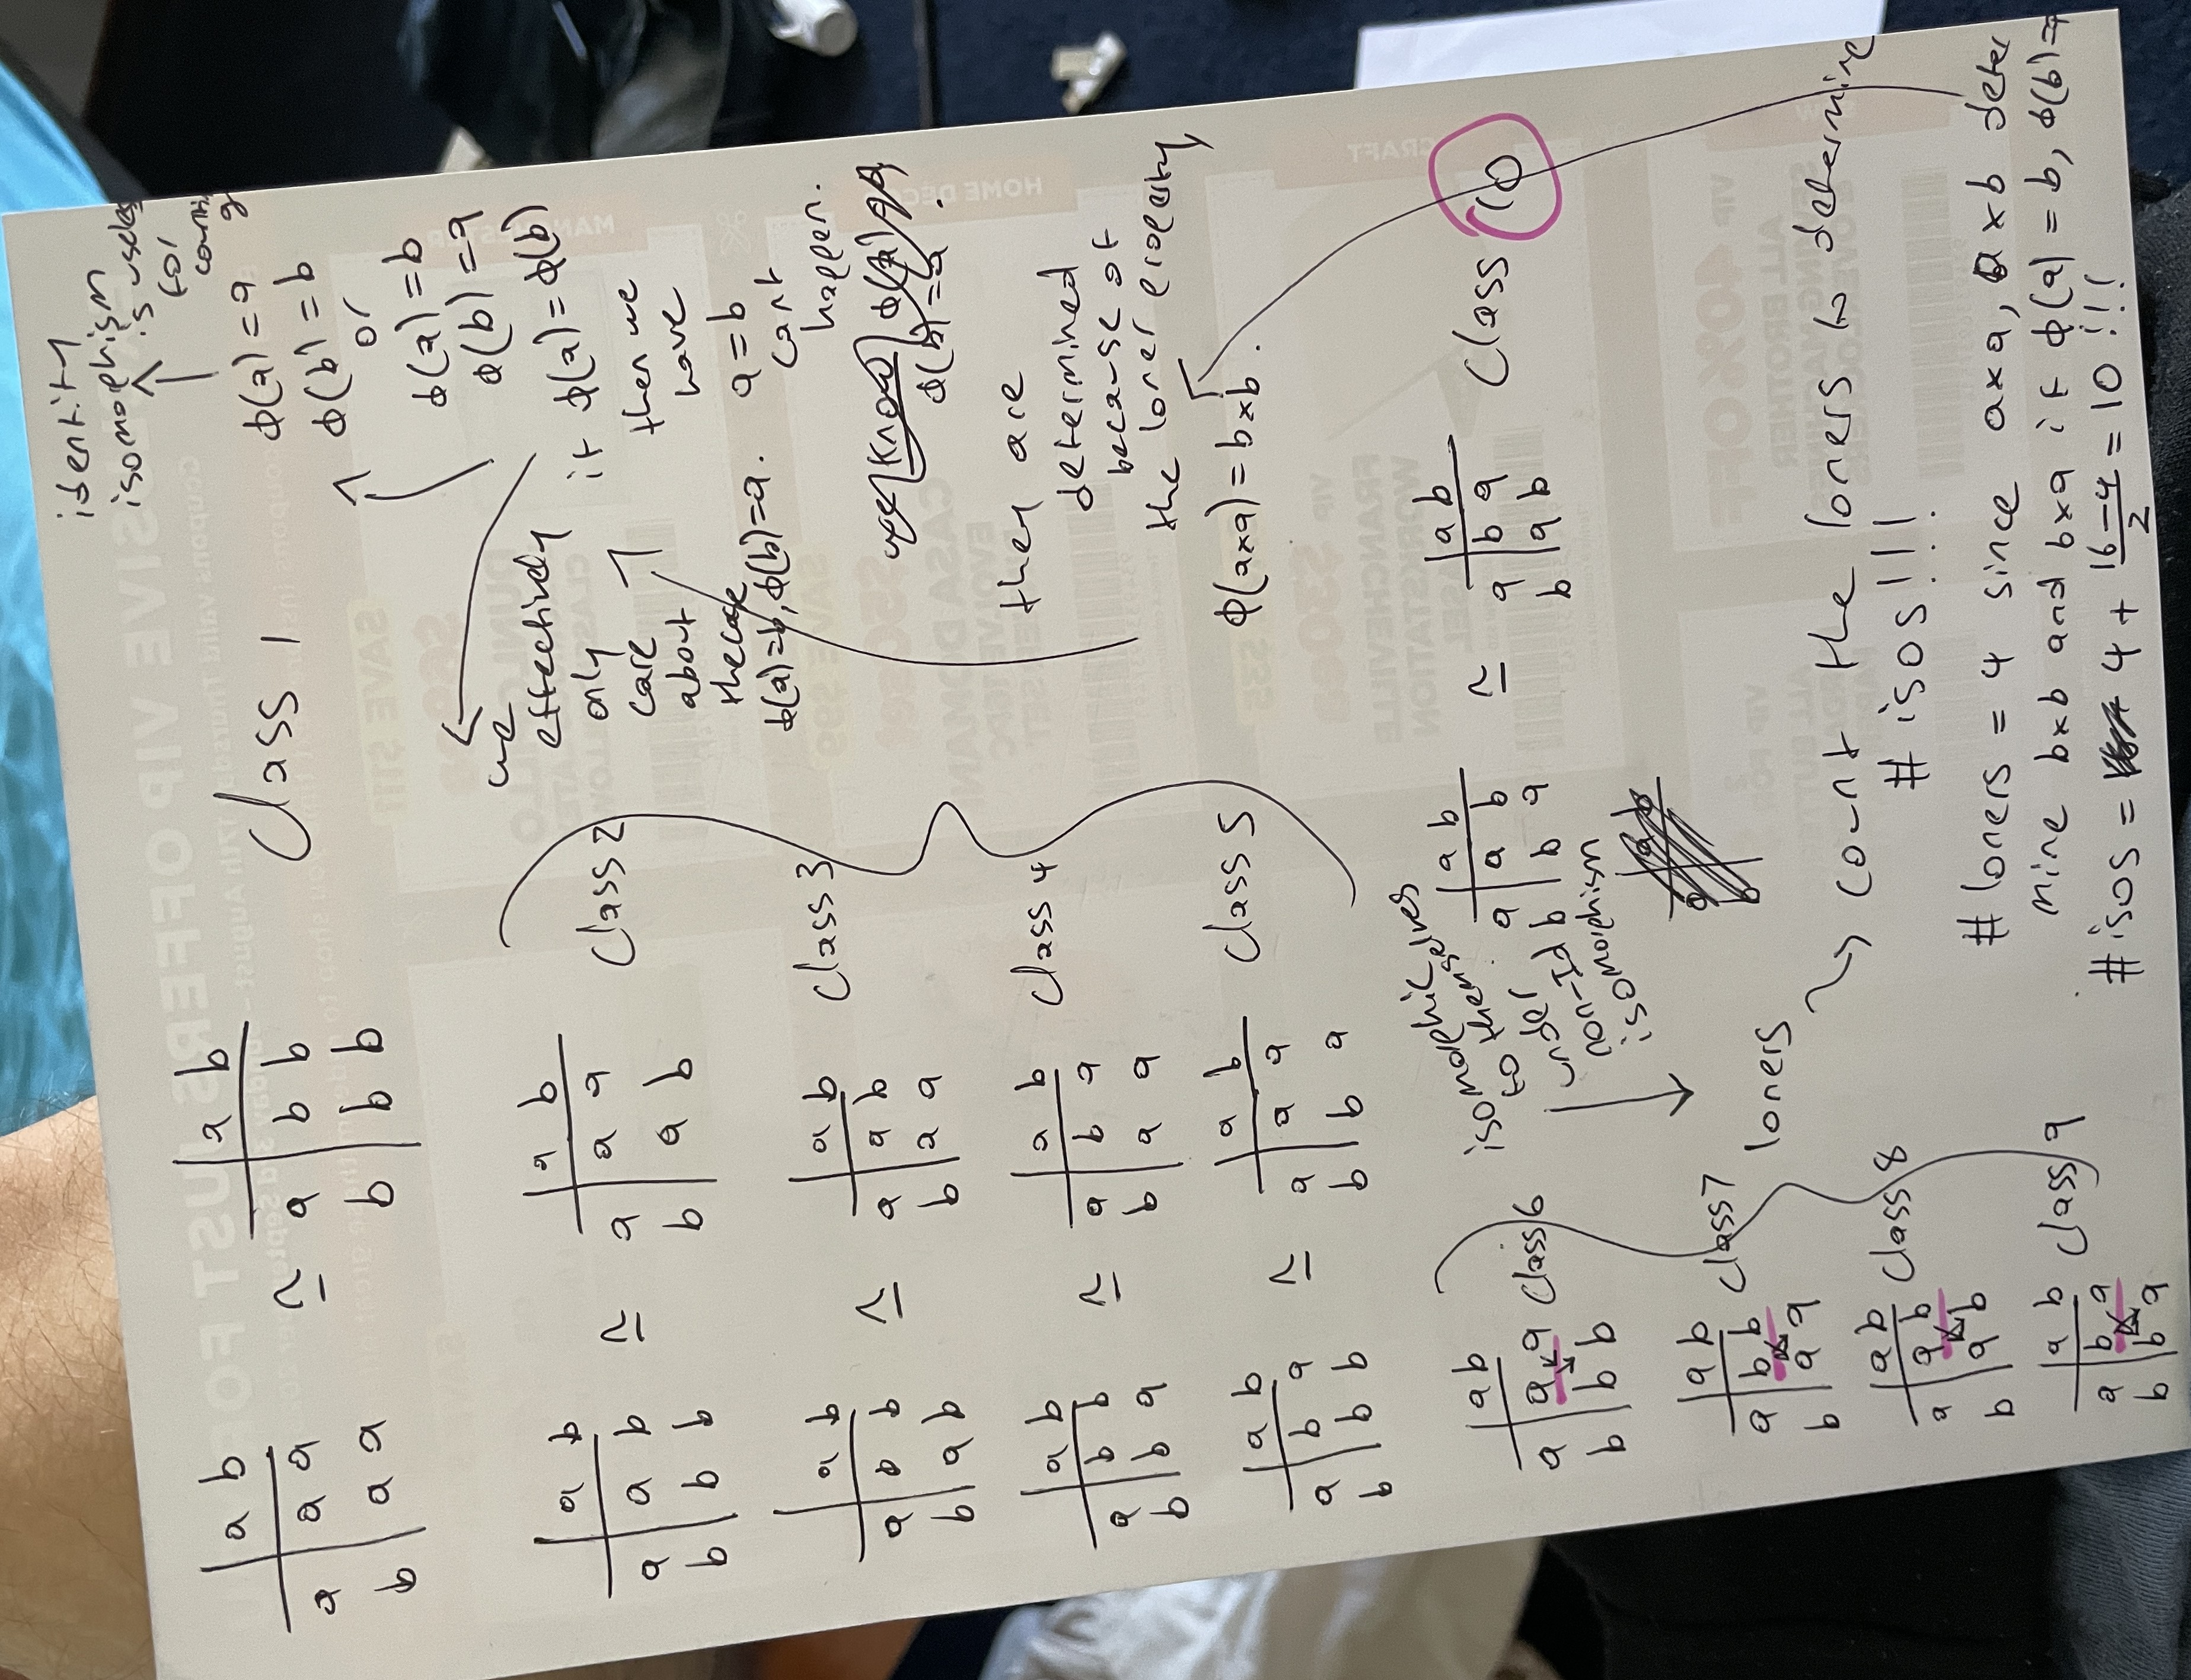
\includegraphics[scale=0.1, angle=-90]{fig/IMG_7272.jpeg}
\end{center}
\section*{Groups}
Here are some:
$$
(U, *) \text{ with } U = \{ z \in \C: |z| = 1 \}, \quad \text{$(U_n,*)$ with } U_n = \{ z \in \C: z^n = 1\}
$$
The invertible $n$ by $n$ matrices and the invertible linear maps on $\R^n$:
$$
\GLM \iso \GL
$$
To get an isomorphism, map an invertible linear function $T: \R^n \to \R^n$ to a matrix using its action on the standard basis.
Left inverses and identities plus associative is enough to define a group.
Identity is a right identity:
\begin{align*}
x + e_L &= e_L + (x + e_L)  \\ &= (x_{LL} + x_L) + (x + (x_L+x)) \\ &= x_{LL} + (x_L+x) + (x_L+x) \\ &=
x_{LL} + e_L + (x_L+x) \\ &= (x_{LL}+x_L)+x \\ &= e_L + x \\ &= x.
\end{align*}
Left inverses are right inverses also,
$$
x + x_L = e_L + x+ x_L = (x_{LL}+x_L) + x + x_L = x_{LL}+e_L+x_L = x_{LL} + x_L = e_L.
$$
\begin{center}
\includegraphics[scale=0.4, angle=-90]{fig/IMG_7275.jpeg}
\end{center}
It's easy to do the same argument with $\phi(e^\pi) = a > 0$.
Bit weirder for $(U,*) \not \simeq (\R^*,*), a^2 = a * a = \phi(e^\pi) * \phi(e^\pi) = \phi(e^{2\pi}) = 1$ but $0 \not \in \R^*$ and $a \neq 1$ since $\phi$ injective and $\phi(e^0) = 1$.
\begin{center}
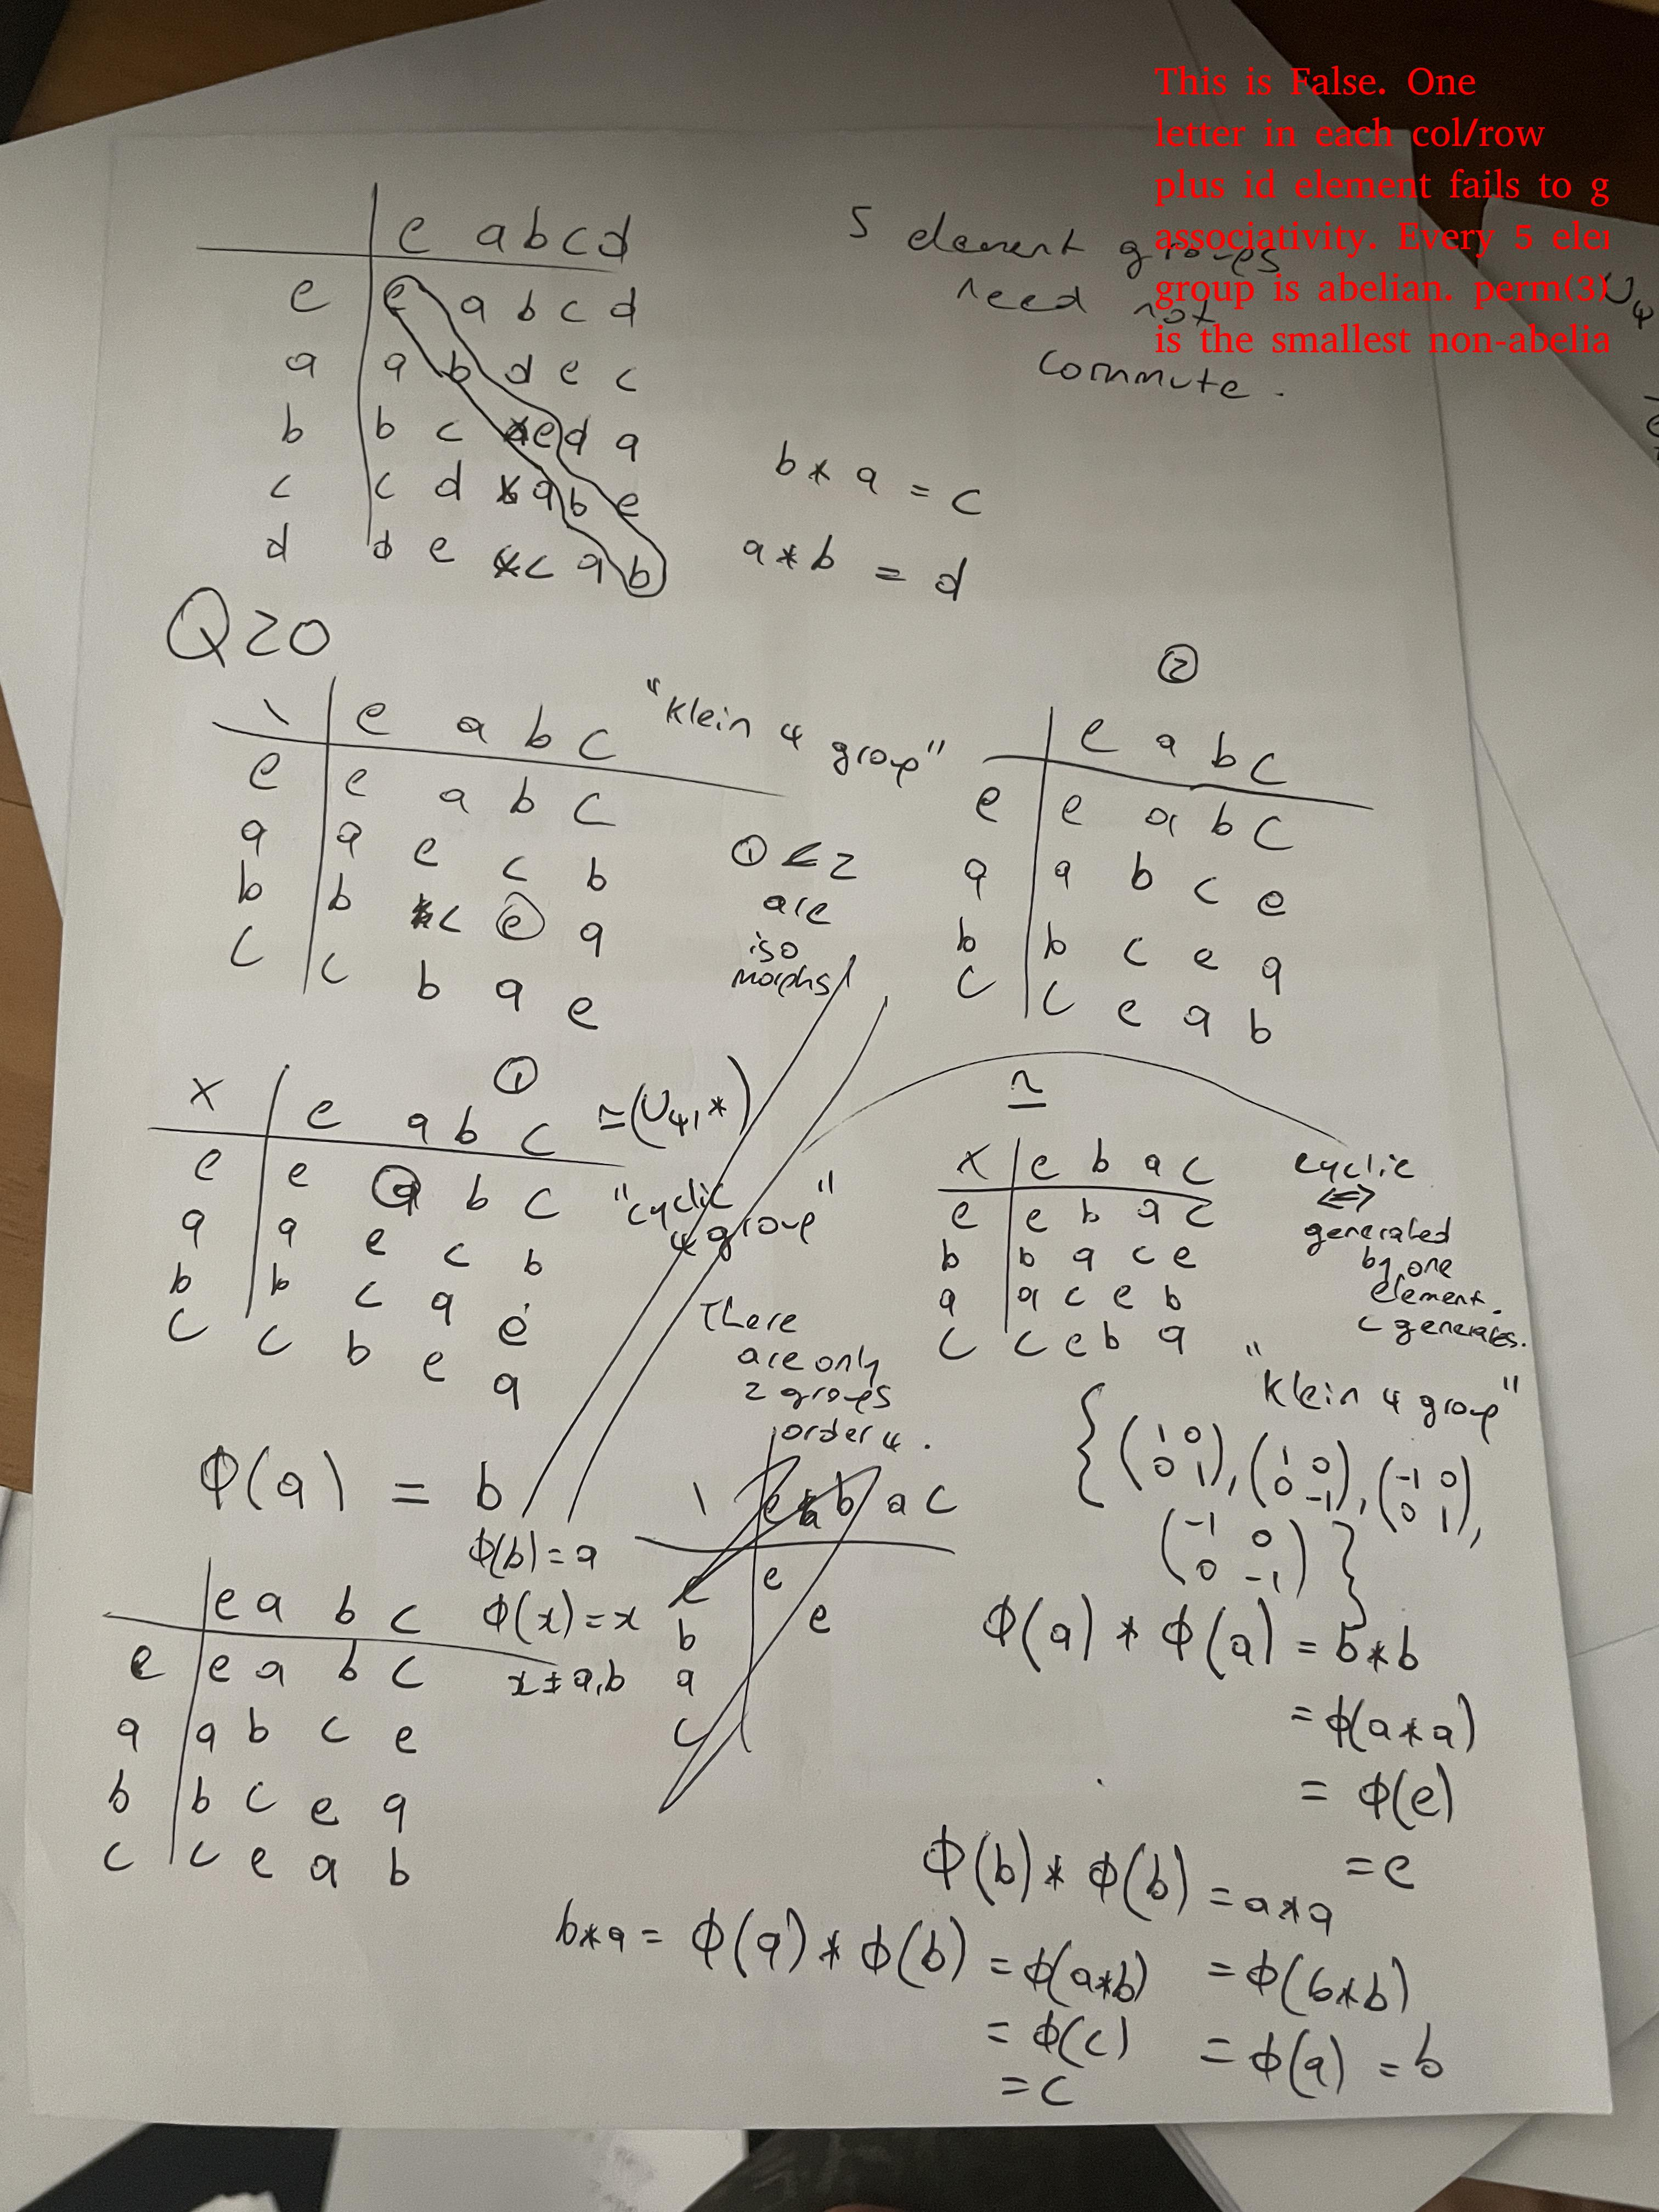
\includegraphics[scale=0.3, angle=-0]{fig/IMG_7284.jpeg}
\end{center}
\section*{Subgroups}
Subgroups are closed, contain identity and inverses. An element $a$ generates $G$ if
the cyclic subgroup $\la a \ra = \{ a^n : n \in \Z \} = G$. We say that $G$ is cyclic if there is some element that generates it.
So obviously $\la a \ra$ is a cyclic group (its always a group). Any group with no proper nontrivial subgroups is generated by every
non identity element (except the trivial group (or not, vacuous??)), so is cyclic.
\newpage{}
\section*{Cyclic Groups}
Subgroup of a cyclic group is cyclic.
\begin{center}
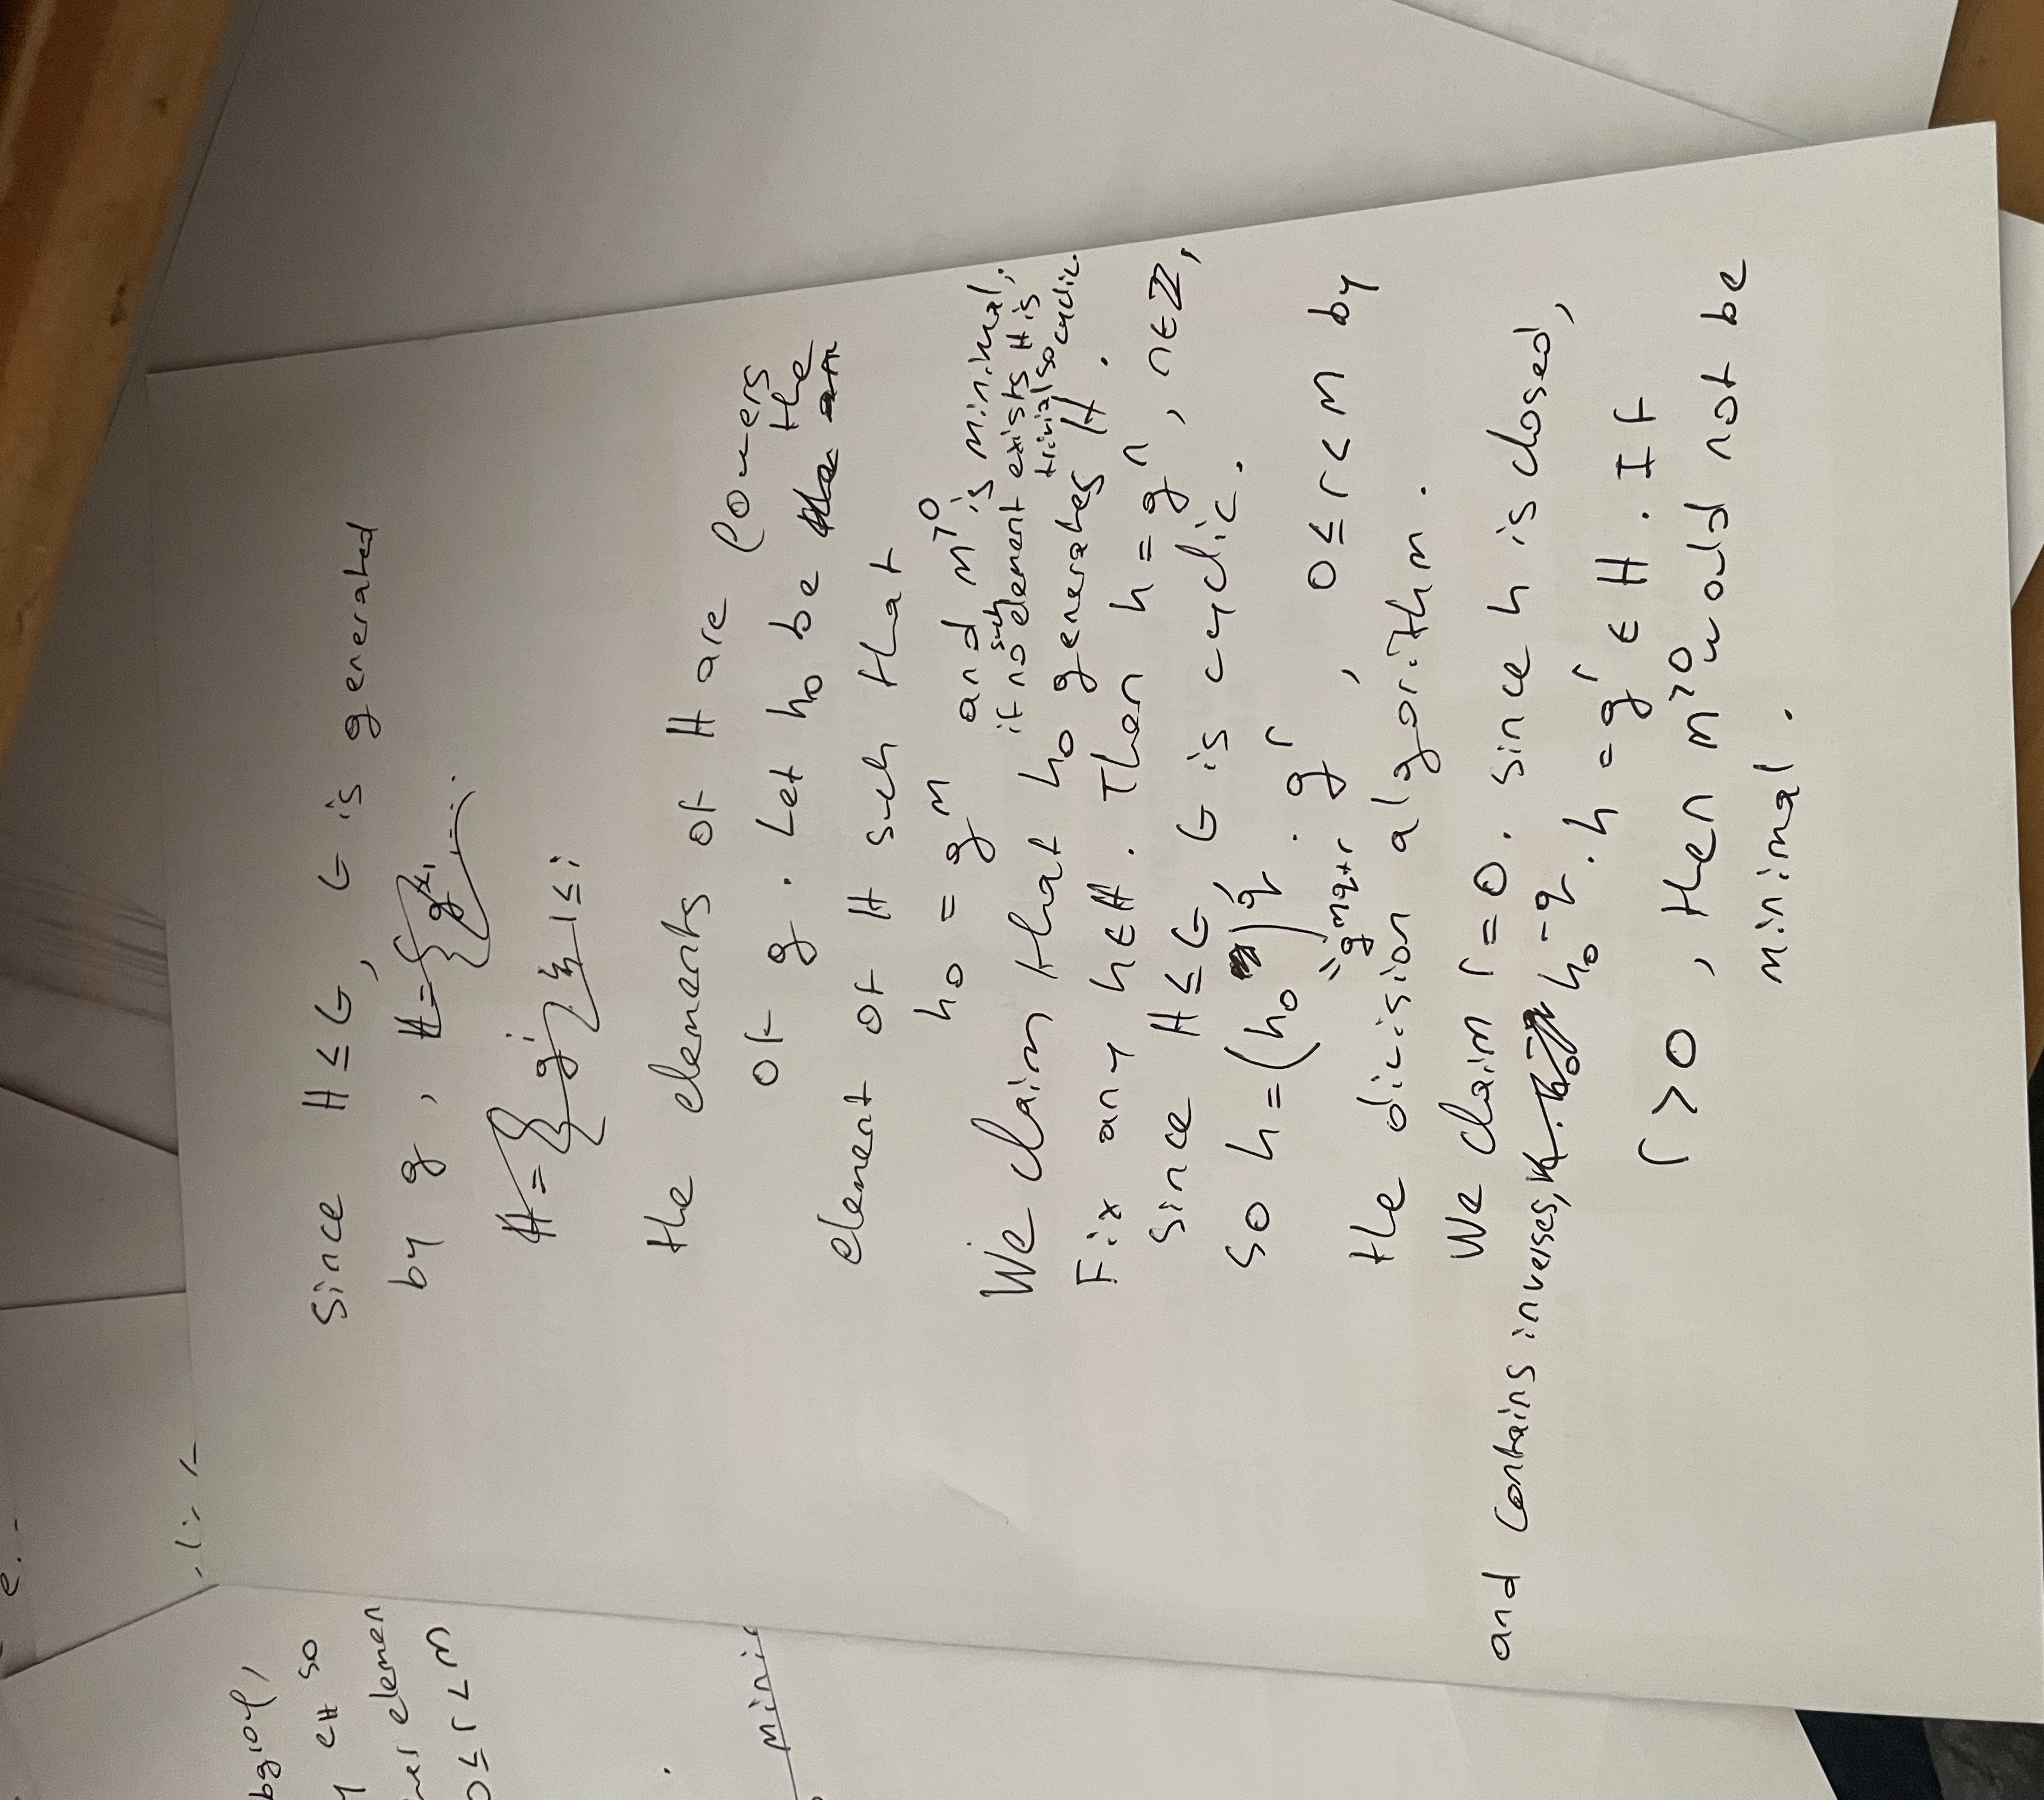
\includegraphics[scale=0.1, angle=-90]{fig/IMG_7322.jpeg}
\end{center}
Pick any subgroup $H$ of the integers under addition. Then $H$ is cyclic, so some $h$ generates $H$. So $h \in \Z$ and we must have $H = h \Z$. \\ \newline
The following is unrelated. A finicky but easy enough proof tells ya that any cyclic group is isomorphic to the integers under addition or the integers under modular addition.
The prior fact about subgroups of $\Z$ characterises subgroups of infinite cyclic groups, since their parents are isomorphic to $\Z$.
\subsection*{The hard bit: Cyclic Subgroups}
\subsubsection*{Defn}
The greatest common divisor of $m,n$ is the generator $d$ of the group $$
\{rm+sn:r,s \in \Z\}
$$
\subsubsection*{Theorem}
Let $G = \la a \ra$ be a cyclic group of order $n$. Then the order of the subgroup generated by
$a^m$ is $n \slash d$. Further, $\la a^m \ra = \la a^p \ra$ iff $\gcd(m,n) = \gcd(p,n)$.
\begin{proof}
Go read the first bit. The iff statement is badly explained. What they are saying is that
$
\{m \in \Z_n:\gcd(m,n) = d\} \subset \la d \ra
$
since $d \vert m \implies m = kd = d^k \in \la d \ra$. Any subgroup
with $n \slash d$ elements contains all elements $a^p$ of $G$ such that
$\gcd(p,n) = d$. In the case of $\Z_n$, this is just integers $p$ with $\gcd(p,n) = d$.
Then $\la a^m \ra$ contains $a^p$ and $\la a^p \ra \subset \la a^m \ra$ and similarly $\la a^m \ra \subset \la a^p \ra$ so $\la a^m \ra = \la a^p \ra$. That is to say, if the gcd's are the same then the subgroups are the same.
If the subgroups are the same, they have the same number of elements, $n \slash d_1 = n \slash d_2 \implies d_1 = d_2$.
\end{proof}
\subsubsection*{Corollary}
For each divisor $d$ of $n$, where $n$ is the order of a cyclic group $G$, there is at most one subgroup of $G$.
\subsubsection*{Corollary}
Given any generator $a$ of $G$ of order $n$, the generators are $a^p$ such that $p$ is coprime with $n$.
\subsubsection*{Defn}
The least common divisor of $m,n$ is the generator of the group $$
\{k \in \Z:m \vert k, \,\, n \vert k\}.
$$
The smallest possible LCM is $mn$ because if $k \vert m$ then $mn = (ak)n = (an)k$ so $k \vert mn$. If $m,n$ are coprime then $m \vert nk$ implies $m \vert k$. In particular,
if $n \vert k$ then $k = qn$ so $m \vert k$ implies $m \vert q$ so that $k = qn = (am)n = a(mn)$, i.e. $mn \vert k$.
\subsubsection*{Theorem}
For positive integers $m,n$
$$
\gcd(m,n) * \lcm(m,n) = mn.
$$
\begin{proof}
Let $\lcm(m,n) = am = bn$. Then $$\frac{mn}{\lcm(m,n)} * a = n,
\quad \frac{mn}{\lcm(m,n)} * b = m$$ so it is a divisor of $a,b$, proving $\frac{mn}{\gcd(m,n)} \leq \lcm(m,n).$
Since $\frac{mn}{\gcd(m,n)}$ is a multiple of both $m$ and $n$,
$\frac{mn}{\gcd(m,n)} \geq \lcm(m,n)$.
\end{proof}
\subsubsection*{Theorem}
Abelian groups with cyclic subgroups $H,K$ of coprime orders $r$ and $s$
have a cyclic subgroup of order $rs$. More generally, there is a subgroup of order $\lcm(r,s)$.
\begin{proof}
We know that $H \cap K$ is a cyclic subgroup. So it must be generated by $x = h^p  = k^q$.
Let $m = |\la x \ra|$. Then $m = r \slash \gcd(p,r) = s \slash \gcd(q,s)$
so $m \vert r$ and $m \vert s$. Then $m \vert \gcd(r,s) = 1$ and $m = 1$. So $H \cap K$ is the trivial group. Now consider the group $Z = \{xy:x \in H, y \in K  \}$ (it is a group since the whole group is Abelian).
Since $H,K$ are finite cyclic groups,  there generators $h,k$ of $H,K$.
We define
a bijection $f:\Z_r \times \Z_s \to Z$, $f(a,b) = h^a k^b$. if $f(a,b) = f(c,d)$,
then $h^{a-b} = k^{d-c} = e$ since $H \cap K  = \{e\}$. So $(a,b) = (c,d)$. Fix $z \in Z$. Then $z = xy = h^a k^b$ where $0 \leq a,b < r,s$ so $f(a,b) = z$. So $f$ is a bijection as asserted. There are $rs$ elements in $\Z_r \times \Z_s$ so the cardinality of $Z$ is $rs$.
We claim that $Z$ is cyclic when $r,s$ are coprime and $gh$ generates $Z$.
Since $r,s$ are coprime there exist integers $m_1,m_2$ so that $1 = m_1 r + m_2s$. Fix $z \in Z$ and write $z = h^ak^b$. Then we have \begin{align*}
(hk)^{bm_1r+am_2s} &= h^{bm_1r+am_2s}*k^{bm_1r+am_2s} \\ &= h^{am_2s}*k^{bm_1r} \\
&= h^{a(1-m_1r)}*k^{b(1-m_2s)} \\
&= h^a*k^b \\ &= z.
\end{align*}
N.B. The Chinese remainder theorem applies here.
\end{proof}
\begin{proof}
Easier proof. Consider $\la hk \ra$. This group is cyclic since it is generated by $hk$.
The order is no more than $rs$, since $(hk)^{rs} = e^s*e^r = e$. Suppose $p < rs$ was the order of $\la hk \ra$.
Then $h^p = k^{-p}$ so that $h^p \in H \cap K$. So $|\la h^p \ra| = d \vert r,s$ which implies $d = 1$, $\la h^p \ra = \{ e \}$. It follows that $h^p = k^p = e$, so $r,s \vert p$ (because they are the orders of $H,K$).
Then $p = ar$, so $s \vert a$ and $p = brs$, $rs \vert p$ which gives a contradiction, $p \geq rs$.
\end{proof}
\subsubsection*{Lemma for General Statement}
Given $r,s$ we can construct coprime $a,b$ so that $a \vert r$, $b \vert s$ and
$ab = \lcm(r,s)$.
\begin{proof}
Write $\lcm(r,s) = d*\frac{r}{d}*\frac{s}{d}$ and $$
d = {p_1}^{a_1} \hdots {p_n}^{a_n} * {q_1}^{b_1} \hdots {q_m}^{b_m}
$$
where $p_i \not \vert r \slash d$ and $q_i \vert r \slash d$.
Then $q_i \not \vert s \slash d$. Consider $$
a = {p_1}^{a_1} \hdots {p_n}^{a_n} * r \slash d,
\quad b = {q_1}^{b_1} \hdots {q_m}^{b_m} * s \slash d.$$
N.B.
if $ab \vert m$ then $a \vert m$,
$b \vert m$ contrapositive is if neither divide $m$ then their product doesn't.
\end{proof}
\subsubsection*{Proof for General Statement}
By the lemma, we can construct coprime divisors $a,b$ of $r,s$
with $ab = \lcm(r,s)$ so that for $r = a\del_1$, $s = b \del_2$
and $\la h^{\del_1} \ra \leq \la h \ra$, $\an{k^{\del_2}} \leq \an{k}$
we have $$|\an{h^{\del_1}}| = r \slash \gcd(\del_1,r) = r \slash \del_1 = a, \quad
|\an{k^{\del_2}}| = s \slash \gcd(\del_2,s) = s \slash \del_2 = b.$$
\subsubsection*{Example}
There is a generator of $\Z_{36}$ because it has
subgroups $\an{2}$,
$\an{3}$ with $12$ and $18$ elements. We write $12 = 6 * 2$ and $18 = 6 * 3$, then separate factors to get $6 = 3 * 2$,
$a = 2 * 12 \slash 6 = 4$, $b = 3 * 18 \slash 6 = 9$ so that $12 = 4 * 3$ and $18 = 9 * 2$.  We take these new factors $3,2$ and raise existing generators to them.
We then have $\an{3^3} = \an{9}$ of order $4$ and $\an{2^2} = \an{4}$ of order 9.
So we can generate $\Z_{36}$ with $9+4 = 13$.
\subsection*{Cayleigh Digraphs}
A group has a correspondence with a digraph with the following properties:
\begin{center}
If ya start at some point and get to some other point in two ways then the two ways will lead to the same destination from any point \\
.\\
Theres one of each generator arc to and from each point. \\
. \\
Some utter nonsense about only one arc going from a to b. \\
. \\
There exists an arc from a to b.
\end{center}
When a generator is an involution we use undirected graph edges.
An obvious implication of this is that in a group, if $a,b,\hdots,x,y$ are involutions then
$(ab \hdots xy)^{-1} = y^{-1}x^{-1} \hdots b^{-1}a^{-1} = yx \hdots ba$.
Pick a vertex $V$. If all pairs of arcs from $V$ go to the same vertex regardless of the order they are chosen then the group is commutative.
\section{Orbits, Lagrange all that Jazz}
\subsection{Perm Groups}
A permutation is a bijection of a set with itself.
If $A,B$ are finite sets of the same order, there is a bijection $f$ and the permutation groups $S_A$ and $S_B$ are isomorphic. The isomorphism is $
\phi \circ \sigma = f \circ \sigma \circ f^{-1}$. Its a homo because
$\phi \circ (\sigma \circ \tau) = f \circ (\sigma \red{\circ} \tau) \circ f^{-1} = f \circ \sigma \red{\circ (f^{-1} \circ f) \circ} \tau \circ f^{-1} = (\phi \circ \sigma) \circ (\phi \circ \tau)$.
\subsubsection{Cayleighs Theorem}
Every group is isomorphic to a subgroup of the group of permutations on the set.
Its not hard just finicky definitions and pedantry in the one to one but only onto the image stuff. Just notice that multiplication by an element permutes the elements in a group.
This allows a well defined function (not an iso) $\phi: G \to S_G$.
The inverse of left multiplication by an element is just left multiplication by the inverse of that element. Multiplication by the identity gives the identity permutation aka the identity map. We have closure, permutations of permutations are permutations. So $\phi(G)$ is a subgroup of $S_G$. The cancellation law says $\phi$ is injective. So $G$ is isomorphic to the subgroup $\phi(G)$ of $S_G$ (weird statement but yeah). \\ \newline
N.B. When computing the order of a permutation, check more than one element... \\ \newline
N.B. Right regular representations use the inverse element not the element itself.
\subsection{Orbits, Cycles, Parity of perms, Alternating Group}
Orbits are the equivalence classes of elements of a group under a permutation. Cycles are permutations with at most one orbit with order greater than 1.
Transpositions swap two elements and fix the rest (cycles of order 2). Theorem: Permutations are composed of either an odd or an even number of these.
The alternating group is the subgroup of $A_n$ of $S_n$ made up of the even permutations. The odd permutations don't form a subgroup because the identity permutation is even.

\begin{center}
\includegraphics[scale=0.5, angle=-90]{fig/IMG_7397.jpeg}
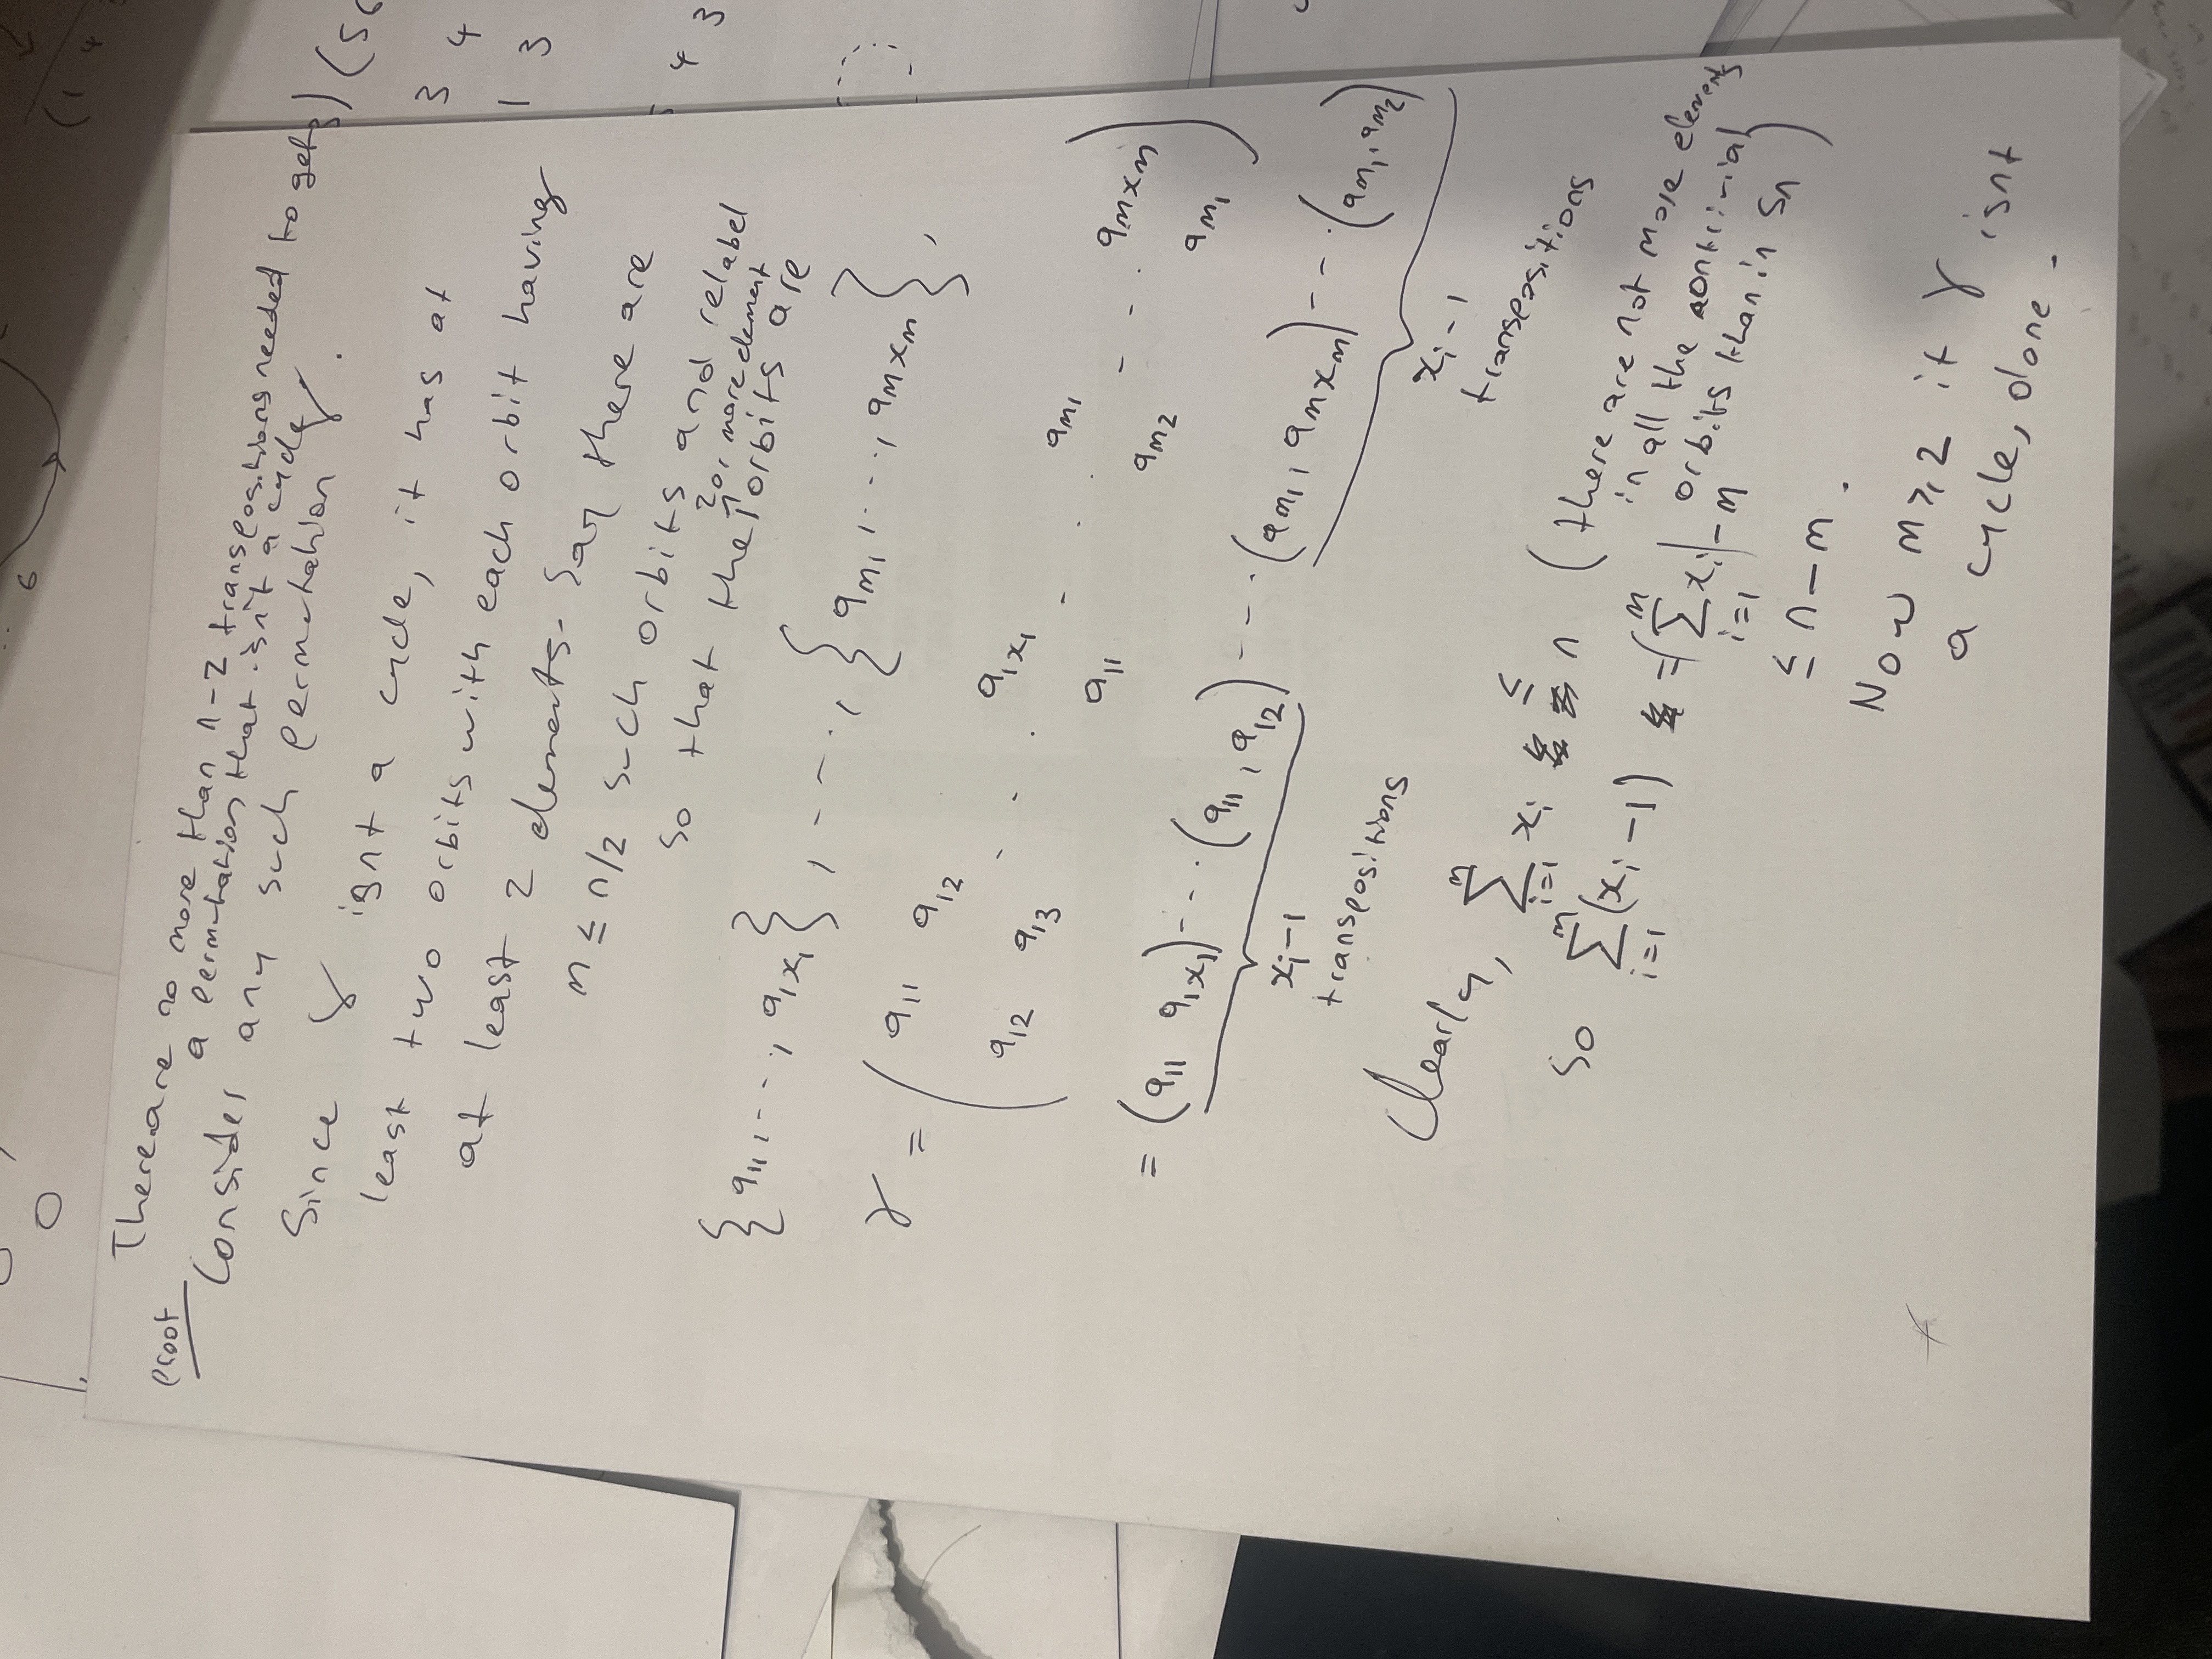
\includegraphics[scale=0.5, angle=-90]{fig/IMG_7398.jpeg}
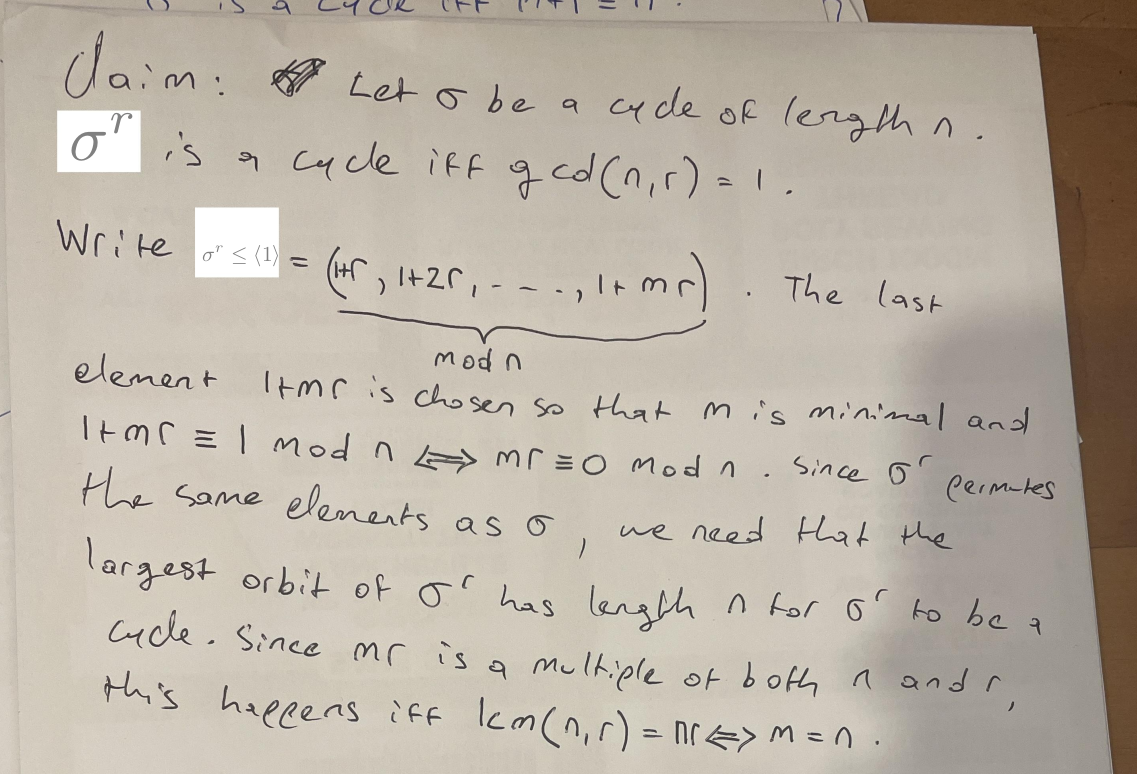
\includegraphics[angle=-0, width=\textwidth]{fig/IMG_7432.jpeg}
\end{center}
\subsection{Cosets, Lagrange's Theorem}
You oughta know why a group of prime order is cyclic. Lagrange's theorem says nothin about infinite order groups.
$(\R,+) \iso (\R^+,\times)$
has no nontrivial finite subgroups, because any $x \neq e$ generates an infinite order subgroup. But $(\R,\times)$ has the subgroup $\{-1,1\}$.
\subsubsection*{Definition}
The index of a subgroup $H \leq G$
is the number of left cosets, $(G:H)$.
\subsubsection*{Lemma}
(Left) cosets of a subgroup are unique.
\begin{proof}
Let $A$ and $B$ be families of left cosets of $H \leq G$, indexed by $a_{\lm}, b_{\del}$.
Pick any $a_{\lm}H \in A$. Since $B$ covers $G$, we have $a_{\lm} \in b_{\del} H$ for some $b_{\del}H \in B$, so we can write $a_{\lm} = b_{\del}h$ for some $h \in H$. We claim that $a_{\lm}H = b_{\del}H$, which implies that $a_{\lm}H \in B$ and furthermore $A \subset B$.
Fix $x \in a_{\lm}H$. Then $x = a_{\lm}h_{x} = b_{\del}hh_{x} \in b_{\del}H$ since $H$ is closed, so $a_{\lm}H \subset b_{\del}H$. Fix $x \in b_{\del}H$. Then $x = b_{\del}h_{\del} = a_{\lm}h^{-1}h_{\del} \in a_{\lm}H$, so $a_{\lm}H = b_{\del}H$. We have shown that $A \subset B$ and a similar argument shows that $B \subset A$, so $A = B$.
\end{proof}
\subsubsection*{Theorem}
Let $G,H,K$ be FINITE groups with $K \leq H \leq G$. Then $(G:K) = (G:H)(H:K)$.
\begin{proof}
Cosets are equivalence classes and $G$ is finite, so write $G = \bigcup_{i=1}^m a_i H$ and  $H = \bigcup_{j=1}^n b_j K$.
Fix $g \in G$. Then write $g = a_i h$ and $h = b_j k$ (being in a coset is an equivalence relation, T0.22 says that eq relations partition a set).
Then $g = a_i b_j k \in \bigcup a_i b_j K$. So $\{ a_i b_jK \}$ covers $G$. We need to show that $\{a_ib_j K\}$ is a partition of $G$. Suppose that $x = a_ib_jk_1 = a_kb_lk_2$ for some $k_1,k_2 \in K$.
Then $x \in {a_i}H \bigcap  {a_k}H$, which is nonempty iff $a_i = a_k$. Use the cancellation law to get $y = b_jk_1 = b_lk_2$. Then $y \in {b_j}K \bigcap  {b_l}K$, which is nonempty iff $b_j = k_l$. So $\{a_ib_jK\}$ is a partition of $G$ into left cosets of $K$.
There's only one of those, so $|\{a_ib_jK\}| = (G:K)$ and clearly $|\{a_ib_jK\}| = mn = (G:H)(H:K)$.
\end{proof}
\section{Homomorphisms, Quotients, Actions and Burnie}
The subgroup generated by the set $\{a_i:i \in I\}$ in $G$ is the
minimal subgroup of $G$ containing $\{a_i:i \in I\}$. If the subgroup is $G$ itself, $\{a_i:i \in I\}$ generates G.
Since the set of finite products of the $a_i$'s is a
subgroup containing $\{a_i:i \in I\}$, it must contain the subgroup generated by them, since that subgroup is minimal.
It is clear that the set of finite products is in the minimal subgroup. So they are equal and we don't need to worry about an element being an infinite product of the generators of a group. A corollary of this is that two homomorphisms that agree on the output of generators of a group agree everywhere.
\subsection*{Factor Groups}
We claim that $\Z_4 \times \Z_2 / \{0\} \times \Z_2  = \Z_4 \times \Z_2 / H \iso \Z_4$. Since the projection
$\phi: \Z_4 \times \Z_2 \to \Z_4$ given by $\phi(a,b) = a$ has kernel $H$ and image $\Z_4$,
\[
\begin{tikzcd}
\Z_4 \times \Z_2 \arrow[rr, "\phi"] \arrow[dr, "\gamma\text{$(x)$ }=\text{ }Hx\text{ homo}"'] & & \phi[\Z_4 \times \Z_2] \\
& \Z_4 \times \Z_2/H \arrow[ur, "\mu(xH)\text{ $=$ }\phi(x)\text{ iso}"']
\end{tikzcd}
\]
\textbf{Fig: Canonical morphisms} \\ \newline
there is a canonical isomorphism from the quotient to $\phi(\Z_4 \times \Z_2) = \Z_4$ via $\mu((a,b)H) = \phi(a,b)$. The moral of the story is that if we can find a homomorphism with a kernel matching our quotient, we can construct an isomorphism with the image of the homomorphism. It doesn't really matter what space we embed $\phi(G)$ in, so long as $\phi$ is still a homomorphism.
We could just as easily have defined $\phi: \Z_4 \times \Z_2 \to \Z_8$, $\phi(a,b) = 2a$. In that case the image of $\phi$ would be a subgroup of $\Z_8$ isomorphic to $\Z_4$.
\subsubsection*{Simple Groups}
A simple group is a NONTRIVIAL group with no proper nontrivial normal subgroups.
Here is an incredibly awkward proof that $A_n, \,\, n\neq 1,2,4$ is simple.
\begin{lemma}
Any permutation can be expressed as a product of disjoint cycles.
\begin{proof}
Let $\sigma \in S_n$. Let $O_1,\hdots,O_m$ be the orbits of $\sigma$, where $1 \leq m \leq n$. For each $1 \leq i \leq m$ define the cycle
$$
\mu_i(x) = \begin{cases}
\sigma(x), \,\, x \in O_i \\
x, \text{ otherwise.}
\end{cases}
$$
Then the cycles are disjoint and $\sigma = \mu_1 \hdots \mu_m$.
\end{proof}
\end{lemma}
\begin{lemma}
Let $N$ be a nontrivial normal subgroup of $A_n$, where $n \geq 5$.
Then $N$ contains a 3-cycle.
\begin{proof}
Pick $\sigma \in N$ with $\sigma \neq \iota$.
Using the lemma, we can write $\sigma$ as a product of disjoint cycles.
If $\sigma$ is itself a 3-cycle, we're done.
If the product contains product of two cycles, where at least one cycle is of length greater than 3, we can write
$$
\sigma = \mu_1 (a_1,\hdots,a_r) \mu_2,
$$
where each factor is disjoint from the others. Since $N$ is normal, $\sigma^{-1} (a_1,a_2,a_3)\sigma(a_3,a_2,a_1) = (a_1,a_3,a_2)$ is in $N$.
If it does not, then there are three cases. Suppose the product is of the form $$
\sigma = \mu_1(a_1,a_2,a_3)\mu_2,
$$
where $\mu_1,\mu_2$ are products of transpositions and the factors are disjoint. Then $\sigma^2 = (a_1,a_3,a_2) \in N$, so $N$ contains a 3-cycle.
Suppose $$\sigma = \mu_1(a_1,a_2,a_3)(a_4,a_5,a_6)\mu_2,$$
where the factors are disjoint.
Let $\tau = \sigma^{-1}(a_1,a_2,a_4)\sigma(a_4,a_2,a_1) = (a_1,a_4,a_2,a_6,a_3) \in N$.
Then $\tau^{-1}(a_1,a_4,a_2)\tau(a_1,a_4,a_2)^{-1} = (a_1,a_2,a_4) \in N$. Finally, suppose $\sigma$
is a product of disjoint transpositions. Then, given that $\sigma$ cannot itself be expressed as a 3-cycle, write $$
\sigma = \mu(a_1,a_2)(a_3,a_4),
$$
where $\mu$ is the product of an even number (possibly zero) of disjoint transpositions.
Let $\tau = \sigma^{-1}(a_1,a_2,a_3)\sigma(a_3,a_2,a_1) = (a_1,a_3)(a_2,a_4) \in N$.
Pick $a_i \in A_n \setminus \{a_1,a_2,a_3,a_4\}$.
Then $\tau (a_1,a_3,a_i) \tau (i,a_3,a_1) = (a_1,a_3,a_i)$, so $N$ contains a 3-cycle.
%$(r,s,i)$, then $\$
\end{proof}
\end{lemma}
\noindent \textbf{The alternating groups are simple for $n \neq 1,2,4$}.
\begin{proof}
The group $A_3$ is of prime order, so simple. If $n \geq 5$, let $N$ be a nontrivial normal subgroup of $A_n$. Then $N$ contains a 3-cycle by the lemma, call it $(r,s,i)$. Fix $j$ between $1$ and $n$.
Then $(r,s,j) = (r,s)(i,j)(r,i,s)(r,s)(i,j) = A (r,s,i)^2 A^{-1} \in N$. It is then possible
to generate any 3-cycle
$(i,j,k)$ with the squaring trick and the computation $(r,i,s)(r,s,k) = (s,k,i)$. Namely,
$(s,j,k)(s,k,i) = (i,j,k)$. Fix $A \in A_n$. Write $A = \del_1 \hdots \del_{k}$ where $$
\del_k = (\del_{k_1},\del_{k_2})(\del_{k_3},\del_{k_4}) = \begin{cases}
\iota, \,\, \text{if } (\del_{k_1},\del_{k_2}) = (\del_{k_3},\del_{k_4}) \text{ as transpositions}, \\
\text{A permutation of } (\del_{k_1},\del_{k_2},\del_{k_3}), \text{ if $|\{\del_{k_1},\del_{k_2}\} \cap \{\del_{k_3},\del_{k_4}\}| = 1$}, \\
(\del_{k_1},\del_{k_2},\del_{k_3})(\del_{k_2},\del_{k_3},\del_{k_4}), \text{ otherwise.}
\end{cases}$$ Then $A$ is a finite product of elements in $N$, so $A_n \subset N$ and $A_n = N$.
\end{proof}
\subsection*{Group Actions are a bit strange}
A $G$-set isomorphism is a bijection $\phi:X \to Y$ with $g\phi(x) = \phi(gx)$.
\begin{theorem}
Suppose $X$ is a \textbf{transitive} $G$-set. Fix $x_0 \in X$ and let $L$ be the set of left cosets of the subgroup $G_{x_0}$ fixing $x_0$.
Then $X$ is isomorphic to $L$.
\end{theorem}
\begin{proof}
Let $\phi: L \to X$ be given by $\phi(\del G_{x_0}) = \del x_0$. Then $\phi$ is well defined, for if
$\del_1 G_{x_0} = \del_2 G_{x_0}$, then $\del_2 = \del_1 g$ and $\del_2 x_0 = \del_1 g x_0 = \del_1 x_0$.
Suppose that $\del_1 x_0 = \del_2 x_0$. Then ${\del_1}^{-1}\del_2 x_0 = x_0$, so ${\del_1}^{-1}\del_2 \in G_{x_0}$. So $\del_2 \in \del_1 G_{x_0}$ and $ \del_1 G_{x_0} =  \del_2 G_{x_0}$ and $\phi$ is injective.
Fix $x \in X$. Since $X$ is transitive, $\exists g \in G$ such that $gx_0 = x$ so that $\phi(gG_{x_0}) = gx_0 = x$, so $\phi$ is a bijection. It is easy to see that $g_1\phi(g_2G_{x_0}) = \phi(g_1g_2G_{x_0})$, so $\phi$ is an isomorphism.
\end{proof}
\begin{cor}
The orbit of element $x \in X$ is $G$-set isomorphic to the collection of
left cosets of the stabiliser subgroup $G_x$.
\end{cor}
\begin{theorem}
Let $X$ be any $G$-set. Then $X$ is \red{(index ignoring $G$-set)} isomorphic to a disjoint union of left coset $G$-sets.
A disjoint union is a cheaty way to write a union of not disjoint sets as disjoint ones by indexing them.
\end{theorem}
\begin{proof}
Since the orbits $O_i$ for $i \in I$ of $X$ are transitive $G$-sets,
the prior theorem says that each orbit
is ($G$-set) isomorphic to
the set $L_{x_i}$ of left cosets of the subgroup fixing some $x_i \in O_i$.
We will denote the isomorphisms between $O_i$ and $L_{x_i}$ by $\phi_i$ for $i \in I$.
We define $L_{x_i}' = \{(x,i): x \in L_{x_i}\}$ so that the
collection of sets $L_{x_i}'$ for $i \in I$ is disjoint.
We claim that $X \iso \bigcup_{i \in I} L_{x_i}'$.
Let $\phi: X \to \bigcup_{i \in I} L_{x_i}'$ be given by $\phi =
\del \circ \psi$ where $\psi: X \to X \times I$ is given by $\psi(x) = (x,j)$ where $j$ is the index of the orbit $O_j$ containing $x$ and $\del: X \times I \to X \times I$ is given by $\del(x,j) = (\phi_j(x),j)$.
It's clear that $\psi$ is injective. Suppose that $\del(a,b) = \del(c,d)$. Then $\phi_b = \phi_d$, and injectivity of $\del$ follows from injectivity of $\phi_b$.
Since $\del$ and $\psi$
are injective, $\phi$ is also. Fix $a \in \bigcup_{i \in I} L_{x_i}'$. Then $a \in L_{x_j}'$ for some $j \in I$, so write $a = (x,j)$ where $x \in L_{x_j}$. Since $\phi_j$ is onto $L_{x_j}$,
we can write $a = (\phi_j(x),j)$ for some $x \in O_j$. Then $\phi(x) = (\del \circ \psi) (x) = \del(x,j) = (\phi_j(x),j) = a$, so $\phi$ is onto.
Now we need to show that $\phi$ is a $G$-set isomorphism. Fix $x \in X$ and $g \in G$ and let $x \in O_j$.
Then since $\phi_j$ is a $G$-set isomorphism and $gx \in O_j$,
$g \phi(x) = g(\phi_j(x),j) \red{\vcentcolon=} (g \phi_j(x),j) = (\phi_j(gx),j) = \phi(gx)$.
% Since the orbits of $X$ are disjoint,
\end{proof}
\begin{theorem}
$H,K$ are conjugate subgroups of $G$ iff the collections of their
left cosets are isomorphic as $G$-sets.
\end{theorem}
\begin{proof}
Reasonably doable.
\end{proof}
\noindent These are weird theorems but they are quite useful.
E.g. How many transitive $S_3$-sets are there and what do they look like? Well theorem 1 says
that any such $S_3$-set $X$ must be isomorphic
to the cosets of a subgroup of $S_3$ that fixes one of the elements in $X$.
There are six subgroups of $S_3$. The two element subgroups of $S_3$ are conjugate subgroups of each other, so
theorem 3 says that the corresponding left coset collections are isomorphic as $S_3$-sets. So we need only consider the actions on the left cosets of the following subgroups: $$
\{\rho_0\}, \,\, S_3, \,\, \{\rho_0,\rho_1,\rho_2\}, \,\, \{ \rho_0, \mu_1\}.
$$
\begin{center}
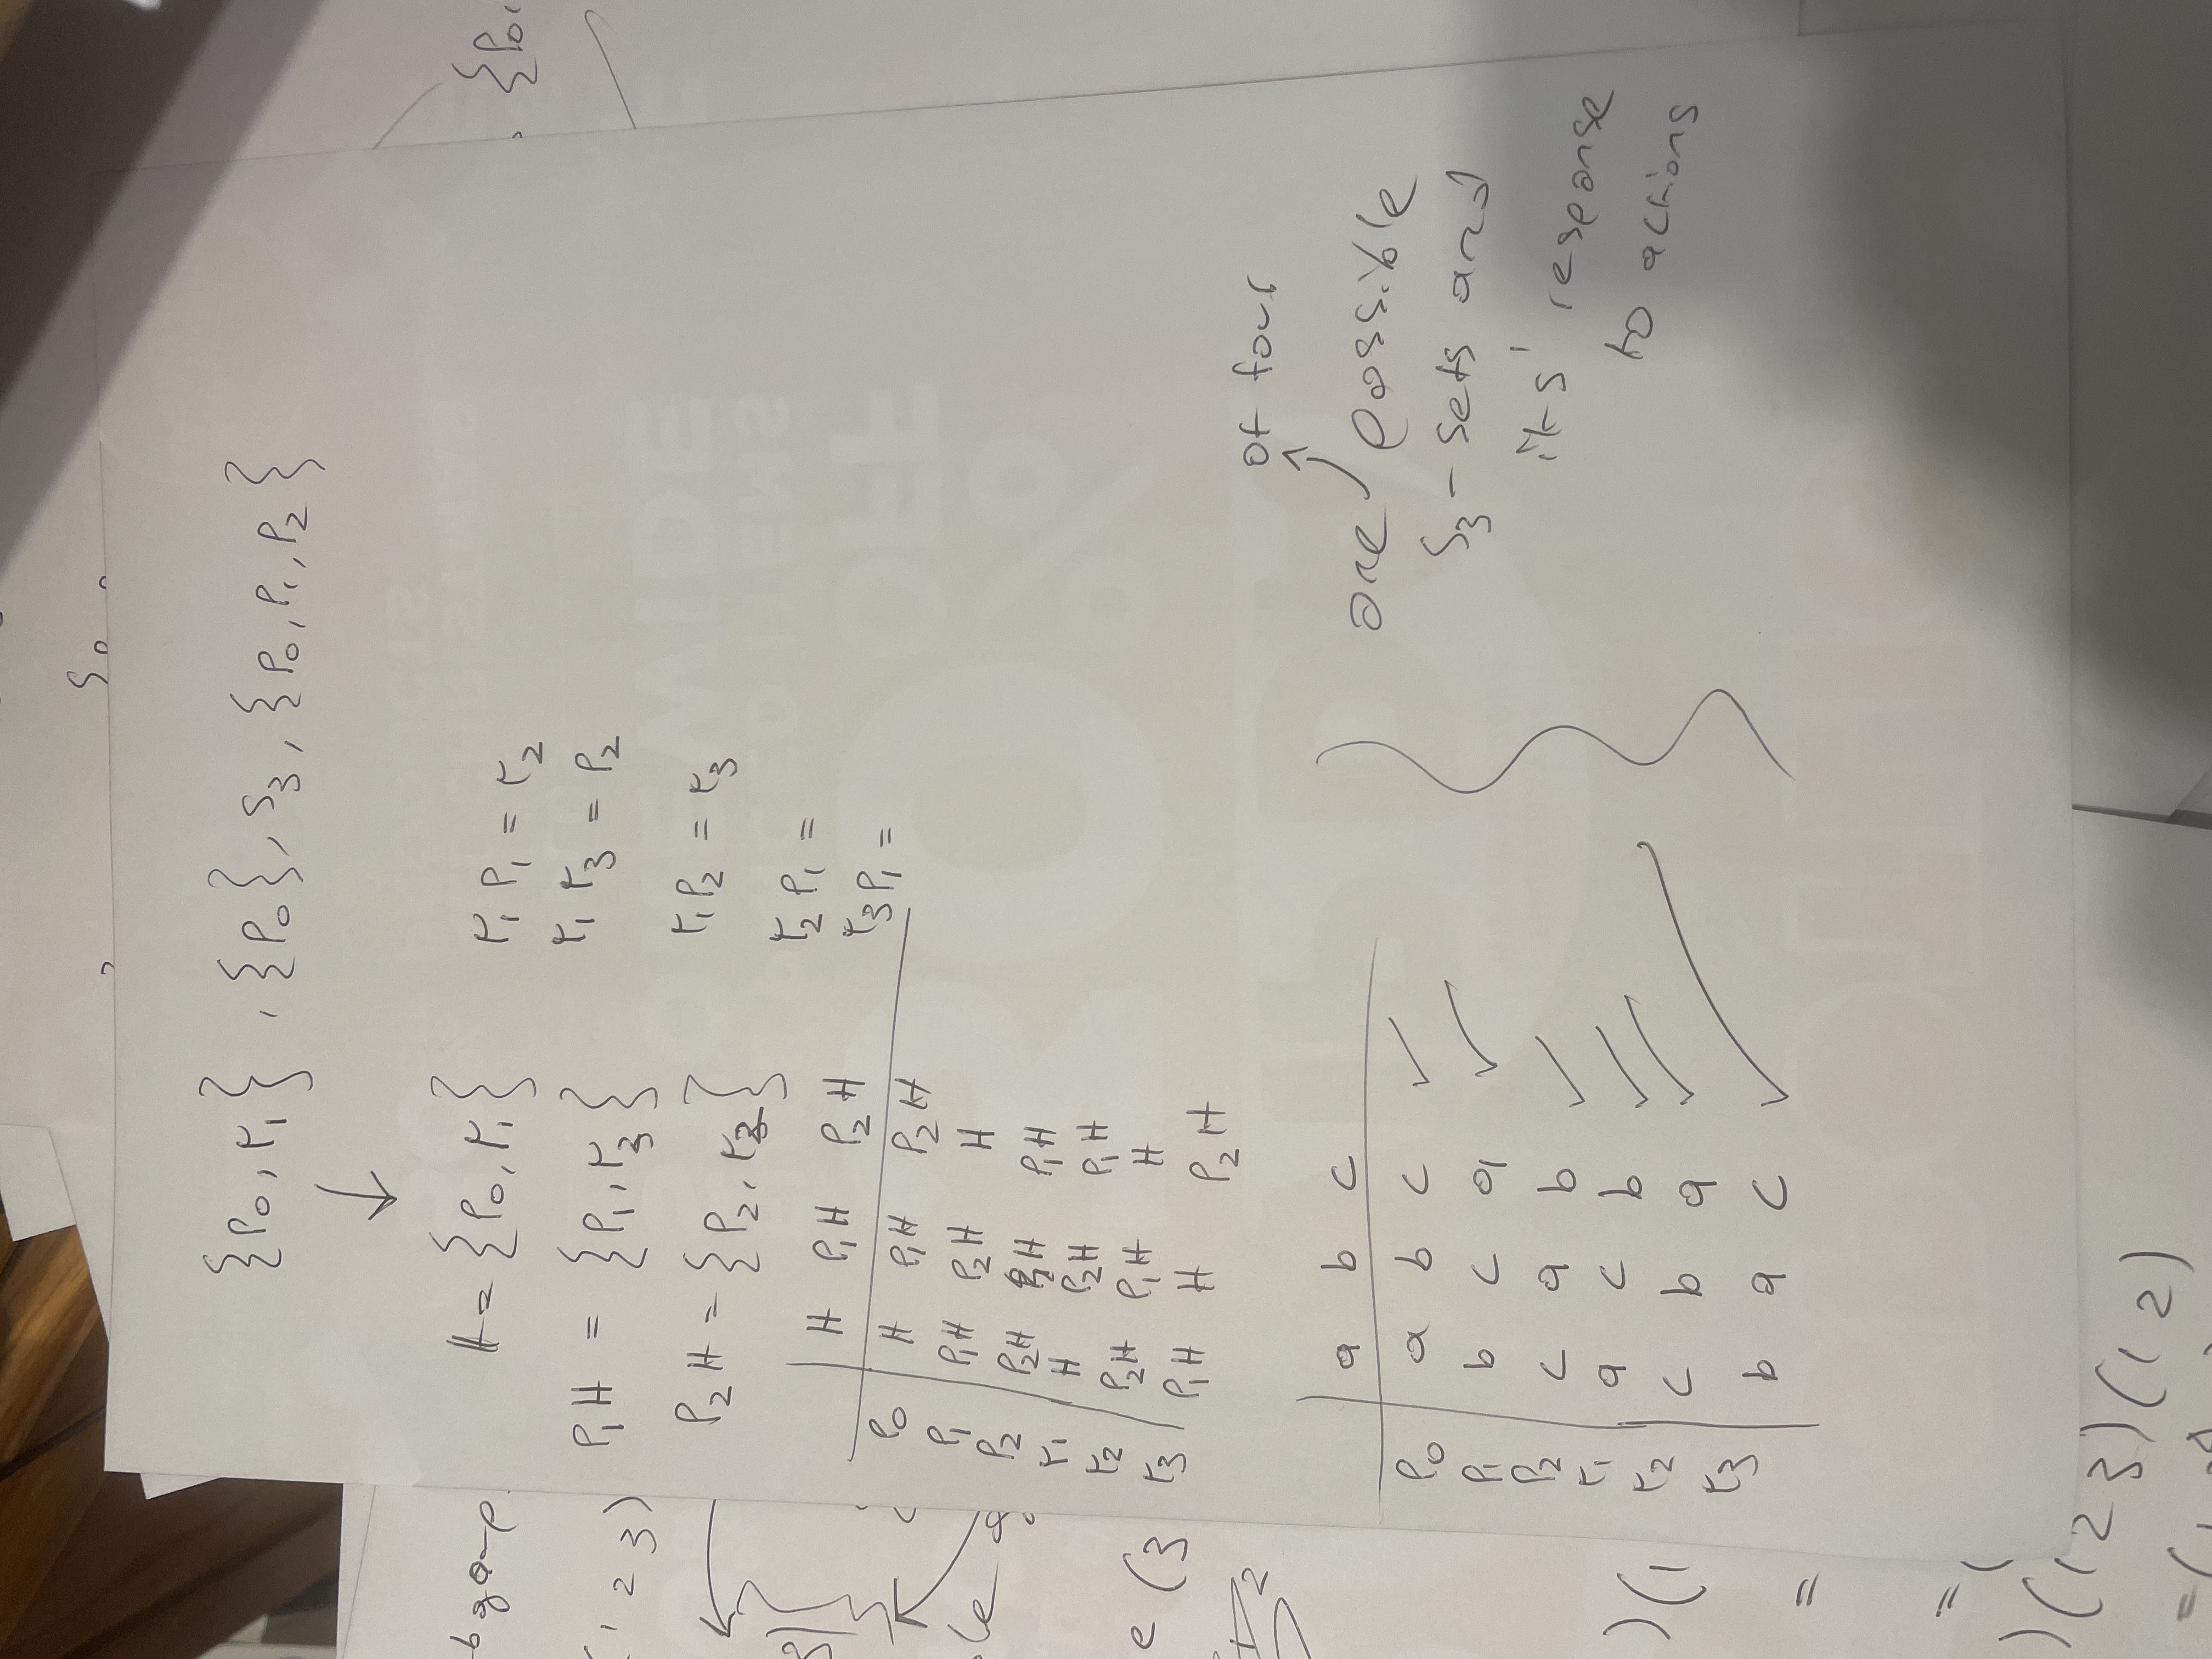
\includegraphics[scale=0.3, angle=-90]{fig/IMG_7469.jpeg}
\end{center}
Two $G$-sets are isomorphic when we can relabel elements in one of their action tables to get the other table.
\newpage{}
\section*{Rings and Fields}
\subsection*{Rings of Polynomials}
We claim that the only units in $D[x]$ are the units of the integral domain $D$.
\begin{proof}
Let $f(x),g(x) \in D[x]$ and write $$f(x) = a_nx^n + \hdots + a_0, \quad g(x) = b_mx^m + \hdots + b_0.$$
Then \begin{align*} fg(x) &= \sum_{j = 0}^{n+m}x^j \sum_{w = 0}^j a_wb_{j-w} \\
& \implies \\
\text{coeff}(x^{n+m}) &= \underbrace{a_0b_{n+m} + \hdots + a_{n-1}b_{m+1}}_0 + a_nb_m + \underbrace{a_{n+1}b_{m-1} + \hdots + a_{n+m}b_0}_0
\end{align*}
Since $D$ is an integral domain and $a_n,b_m \neq 0$, the product $a_nb_m \neq 0$. In particular, if $n+m \geq 1$ then $fg(x) \neq 1$. The contrapositive is that if $fg(x) = 1$, then $n+m < 1 \iff n = m = 0.$
\end{proof}
More or less the same argument says that $D[x]$ is itself an integral domain.
\begin{theorem}
Suppose that $F$ is a FINITE field. Then $p_F = F^F$.
\end{theorem}
\begin{proof}
Well $f \in F^F$ is uniquely defined by its values on $\{a_1, \hdots, a_n\} = F$. So for $g(x) = \sum_{i=1}^n c_i g_i(x)$, where
$$
c_i = f(a_i)(a_i-a_1)^{-1}\hdots (a_i - a_{i-1})^{-1} \quad (a_i - a_{i+1})^{-1} \hdots (a_i-a_n)^{-1} \in F
$$
and
$$
g_i(x) = (x-a_1)\hdots(x-a_{i-1})\quad (x-a_{i+1})\hdots(x-a_n) \in p_F,
$$
we have $g(a_1) = g_1(a_1) + 0 \hdots + 0 = f(a_1) * 1 * \hdots * 1 = f(a_1)$ and so on for $a_2, \hdots,a_n$ by construction.
So $f(a) = \phi_a(g(x)) \in p_F$.
\end{proof}
\subsection*{Factorisation of Polynomials Over a Field}
N.B. reducible doesn't mean zeros exist, e.g. $(x^2+1)^2$ is reducible.
\begin{theorem}
Deg 2,3 poly's are reducible iff they have zeros.
\end{theorem}
\begin{proof}
It's not deep.
\end{proof}
\begin{theorem}
A polynomial of degree $m$ has at most $m$ zeros.
\end{theorem}
\begin{cor}
Any FINITE subgroup $G$ of the multiplicative group of a field $F$ is cyclic.
\end{cor}
\begin{proof}
Well $G \iso \Z_{d_1} \times \hdots \times \Z_{d_n}$ where $d_i$ are powers of primes. Let $m = \lcm(d_1,\hdots,d_n)$. Then $|G| \geq m$. Since $d_i \vert \,\,|G|$, $g^{|G|} = 1$, since each component evaluates to the multiplicative identity. So every $g \in G$ is a solution to $x^m-1 = 0$ in $F$.
Theorem says $m \geq |G|$, we then have $m = |G|$, so $d_i$ are (powers of) unique primes. So $G \iso \Z_{|G|}$ which is cyclic.
\end{proof}
\begin{lemma}
For any non-constant polynomials $$p(x) = a_{m+k}x^{m+k}+\hdots+a_0,\quad g(x) = b_mx^m+\hdots+b_0$$
in a commutative ring with unity where $b_m$ is a unit,
we can write
$$
p(x) = g(x)q(x)+r(x),
$$
where $r(x) = 0$ or $r(x)$ has a smaller degree than $g(x)$.
\end{lemma}
\begin{proof}
Read the book 23.1.
\end{proof}
\begin{theorem}\label{thm:factor}
A polynomial $p(x)$ in a commutative ring with unity $R[x]$
has a zero iff the zero factors into $p(x)$.
\end{theorem}
\begin{proof}
If $(x-m)$ is a factor then it is obvious that $m$ is a zero.
If $m$ is a zero, then use the lemma to write $$
p(x) = (x-m)q(x)+r(x).
$$
Then $r(x)=0$ or has degree zero but that can't happen since $p(m) = 0$.
\end{proof}
\begin{theorem}\label{thm:rational-root}
A primitive polynomial $f(x) \in \mathbb{Z}[x]$ is reducible iff $f(x)$ is reducible in $\mathbb{Q}[x]$. Primitive means the gcd of the coefficients is $1$.
\end{theorem}
\begin{theorem}
The Eisenstein criterion says that if $a_n \neq 0 \in \Z_p$ and $a_0 \neq 0 \in \Z_{p^2}$
while $a_{n-1},\hdots,a_0 = 0 \in \Z_p$, then $f(x) \in \Z[x]$ is irreducible over $\mathbb{Q}$.
\end{theorem}
\begin{proof}
Let $d = \gcd(a_n,\hdots,a_0)$. Then $f(x) \slash d$ is primitive and so Theorem~\ref{thm:rational-root} says we can work in $\Z[x]$.
Let $$
f(x) \slash d = (b_rx^r+\hdots+b_0)(c_sx^s+\hdots+c_0).
$$
Since $d \vert a_0,a_n$, $d \neq 0 \in \Z_{p^2}, \Z_p$ and so $d$ is a unit in the ring $\Z_{p^2}$.
We can use cancellation to see that $$b_0c_0d = a_0 = 0 \in \Z_{p^2} \iff b_0c_0 = 0 \in \Z_{p^2}.$$
In particular, the condition that $a_0 \neq 0 \in \Z_{p^2}$ tells us that one of $b_0,c_0$ must not be equal to zero in $\Z_{p}$. Let's go ahead and assume it's $b_0$.
Then let $m$ be the smallest integer such that $c_m \neq 0 \in \Z_p$.
Then $$
a_m = db_0c_m + db_1c_{m-1} + \hdots +
\begin{cases}
db_r c_{m-r} \text{ if $m > r$} \\
db_{s}c_{0} \\
\end{cases}
$$
Since $d,b_0,c_m \neq 0 \in \Z_p$ while the terms that follow contain $c_{m-i}$ which are zero, $a_m \neq 0 \in \Z_p$ and so $m=n=s$ and $r=0$. So $$
f(x) = db_0 (c_nx^n+\hdots+c_0),
$$
only trivial factorisations can occur and $f(x)$ is irreducible.
\end{proof}
Eisenstein is more usable if we consider $f(x+a)$ and reversed coefficient $f(x)$ but its not the best for random polynomials.
\begin{cor}
The Cyclotomic polynomials $\Phi_p(x) = \frac{x^p-1}{x-1} = x^{p-1} + \hdots + 1$ are irreducible because Eisenstein says that $\Phi_p(x+1)$ is irreducible. Actually $p$ need not be prime, the roots are roots of unity.
\end{cor}
\begin{theorem}
If $f(x) = x^n + a_{n-1}x^{n-1}+\hdots + a_0 \in \Z[x]$ with $a_0 \neq 0$ has a rational zero,
it has an integer zero $m$ dividing $a_0$.
\end{theorem}
\begin{proof}
Well the greatest common divisor of the coefficients is one so we are allowed to use
Theorem~\ref{thm:rational-root}. Then Theorem~\ref{thm:factor} says
$$
f(x) = (x-m)(x^{n-1}+\hdots-m^{-1}a_0).
$$
\end{proof}
The whole shebang about Theorem~\ref{thm:rational-root} is only needed because we are talking about rational zeros.
For $\Z_n[x]$, we would see that if $m$ is a zero then $(x-m)$ is a factor and
$m$ must divide $a_0$ in $\Z_n$. N.B.
however that divisors of $a_0$ in $\Z_n$ need not be divisors of $a_0$ in $\Z$.
E.g. $1,2,4,5$ are divisors of $4 \in \Z_6$ and $5$
is a zero of $x^2+5x+4$ but $5 \not \vert 4 \in \Z$. For $\Z_p$ there is no free lunch, every nonzero element is a divisor of $a_0$.
\end{document}
